\documentclass[notitlepage, 12pt]{report}
\usepackage[utf8]{inputenc}
\usepackage[T1]{fontenc} % makes the angle brackets display properly
\usepackage[margin=1in]{geometry}
\usepackage{graphicx}
\usepackage{enumitem}
\usepackage{helvet}
\usepackage{wrapfig}
\usepackage{float}
\usepackage[export]{adjustbox}
\usepackage{fontspec}
\usepackage{xcolor}
\usepackage{titling} % https://tex.stackexchange.com/questions/591/removing-vertical-space-inside-maketitle/593
\usepackage{authoraftertitle}
\usepackage{xltabular}
\usepackage[document]{ragged2e}
\usepackage[font=small,labelfont=bf]{caption}

\renewcommand{\familydefault}{\sfdefault}

\graphicspath{{images/}}

\newcommand{\code}[1]{\texttt{#1}}

\title{Criterion C: Development}
\definecolor{msblue}{HTML}{5AB5D8}

\begin{document}
% Title
\centerline{\textcolor{msblue}{
		\fontspec{Cambria}\textbf{\fontsize{13}{13}\MyTitle}
	}}
\bigskip

My timeblocker program is written using a client-server architecture. The client is a website frontend written using HTML, CSS, and TypeScript (a statically-typed superset of JavaScript). The server is a Node.js backend with a PostgreSQL database.

\section*{Frontend}
The frontend is a single-page application built with Vue, a JavaScript framework for building user interfaces. The files for the frontend are all contained within the `frontend/` folder.

\section*{Significant files/folders:}
\begin{xltabular}{\textwidth}{
		@{}
		p{0.3\textwidth}
		X
	}
	% https://tex.stackexchange.com/a/57709
	\centerline{\adjustbox{valign=t}{
			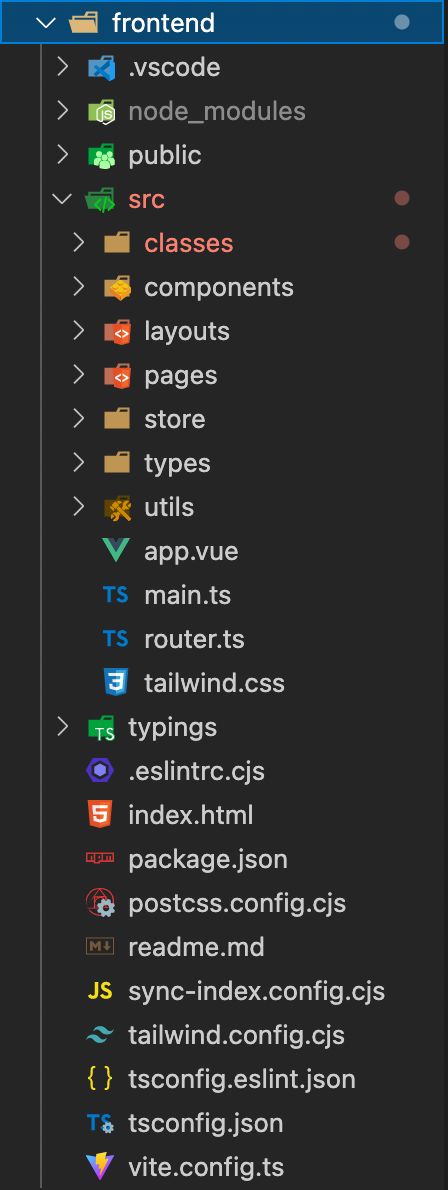
\includegraphics[width=0.3\textwidth]{frontend-files.png}
		}}
	&
	\begin{itemize}[label={}, leftmargin=5pt]
		\item \textbf{public:} Assets that are hosted on the website as-is (e.g. the favicon).
		\item \textbf{src/:} The main website source code.
		      \begin{itemize}[label={}]
			      \item \textbf{classes/:} Frontend’s OOP classes.
			      \item \textbf{components/:} Vue components.
			      \item \textbf{layouts/:} UI templates reused across multiple pages.
			      \item \textbf{pages/:} Website pages.
			      \item \textbf{store/:} Global data store.
			      \item \textbf{types/:} TypeScript types.
			      \item \textbf{utils/:} Various utility functions.
			      \item \textbf{app.vue:} Main Vue component.
			      \item \textbf{main.ts:} Entrypoint for website scripts.
			      \item \textbf{router.ts:} Website routing configuration.
			      \item \textbf{tailwind.css:} Loads TailwindCSS styles.
		      \end{itemize}
		\item \textbf{index.html:} Website entrypoint.
		\item \textbf{Configuration files (*.cjs, *.json, vite.config.ts):} Configuration files for various frontend development tools.
	\end{itemize}
\end{xltabular}
\section*{Development}
To develop my program, I used various build tools from the JavaScript ecosystem.
For the frontend, I used Vite, a build tool that uses a feature called ``Hot Module Reload'' that allows me to update the site without needing to refresh the page.

\section*{User Interface}
\begin{xltabular}{\textwidth}{
		@{}
		p{0.3\textwidth}
		X
	}
	\centerline{\adjustbox{valign=t}{
			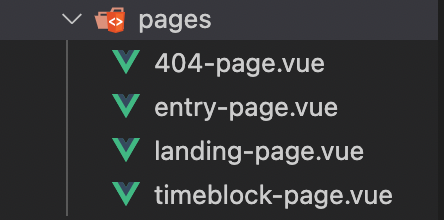
\includegraphics[width=1\linewidth]{frontend-pages-folder.png}
		}}
	&
	The code responsible for the user interface is stored under the src/pages folder.
	The \code{.vue} file extension indicates Vue Single-File Components, or SFCs for short.
	These files contain all the necessary HTML, CSS, and JavaScript to render a component part of a dynamic user interface.
\end{xltabular}

\vspace{10pt}

% https://tex.stackexchange.com/questions/205086/do-not-indent-a-tabular
\noindent\begin{xltabular}{\textwidth}{
		@{}
		X
		p{0.6\textwidth}
		@{}
	}
	In each Vue SFC, there are three root tags: the \code{<script>} tag, the \code{<template>} tag, and the \code{<style>} tag. The \code{<script>} tag contains the JavaScript/TypeScript code that is executed when the component is initialized for the first time. The \code{<template>} tag contains the HTML that defines the structure of the component, and the \code{<style>} tag contains the CSS that is used to style the component.
	&
	\centerline{\adjustbox{valign=t}{
			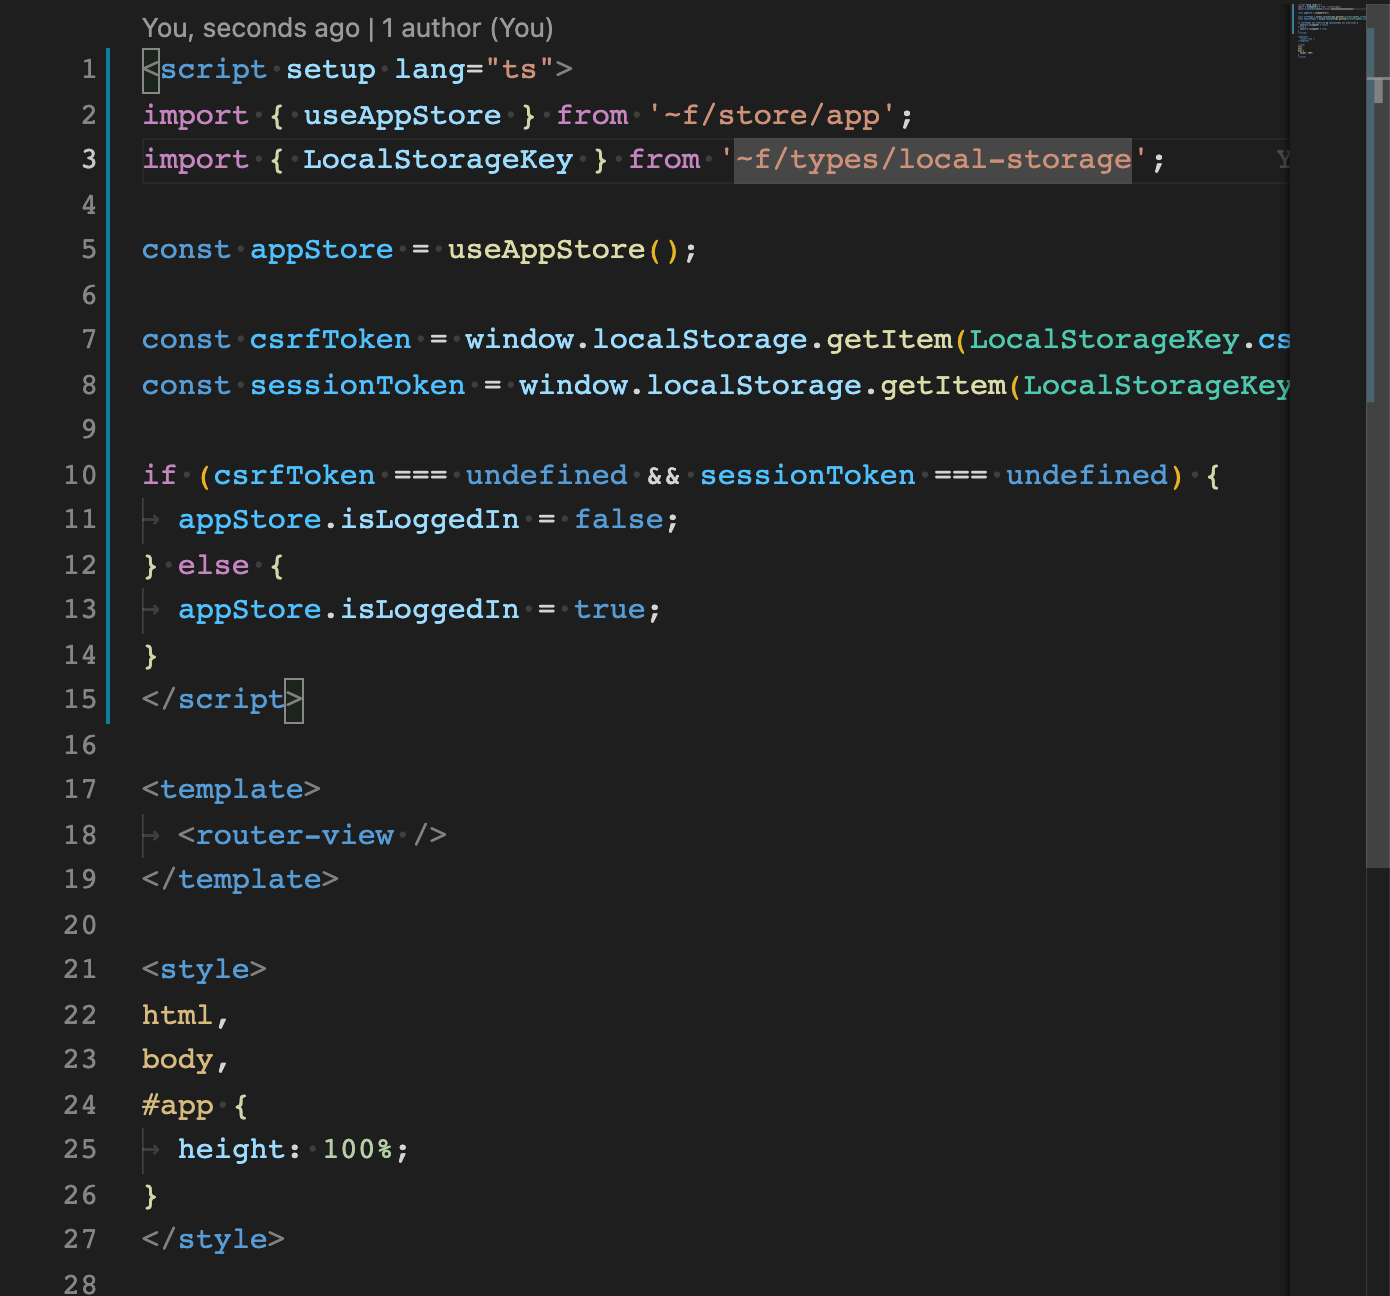
\includegraphics[width=0.6\textwidth]{frontend-vue-sfc.png}
		}}
\end{xltabular}

Most of the SFCs don't contain a \code{<style>} tag because the CSS styles are primarily contained within the HTML using TailwindCSS's utility classes. TailwindCSS is a CSS framework that provides flexible utility classes for making it easier to style HTML. In addition, I used a Tailwind library known as daisyUI that provides out-of-the-box styled components for common HTML components.

\section*{Landing Page}

\begin{figure}[H]
	\caption{A screenshot of Timeblocker's landing page.}
	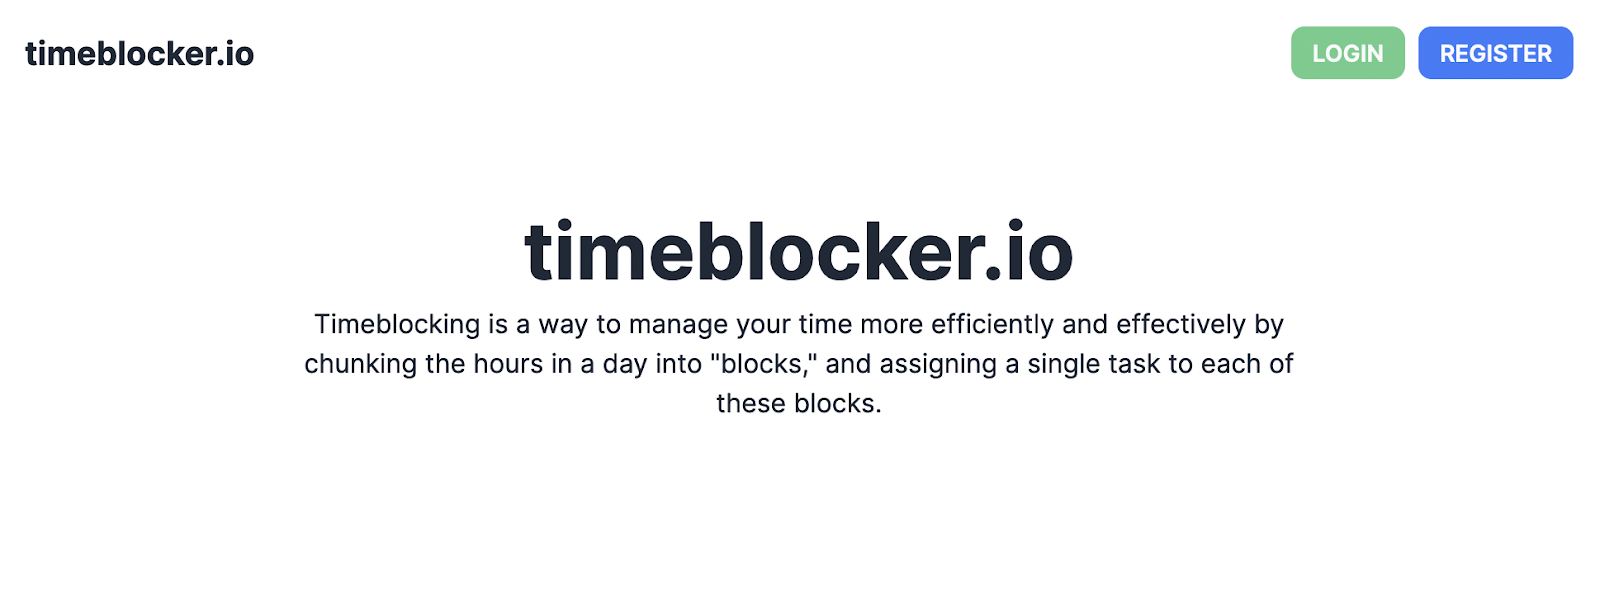
\includegraphics[width=\textwidth]{frontend-landing-page.png}
\end{figure}

\newpage

To build the landing page, I used Vue's \code{v-for} feature: instead of copy-pasting my HTML code three times, I defined the information needed to render each feature in my JavaScript and used \code{v-for} to render multiple HTML elements:

\begin{figure}[H]
	\caption{Storing the features and descriptions in a JavaScript array.}
	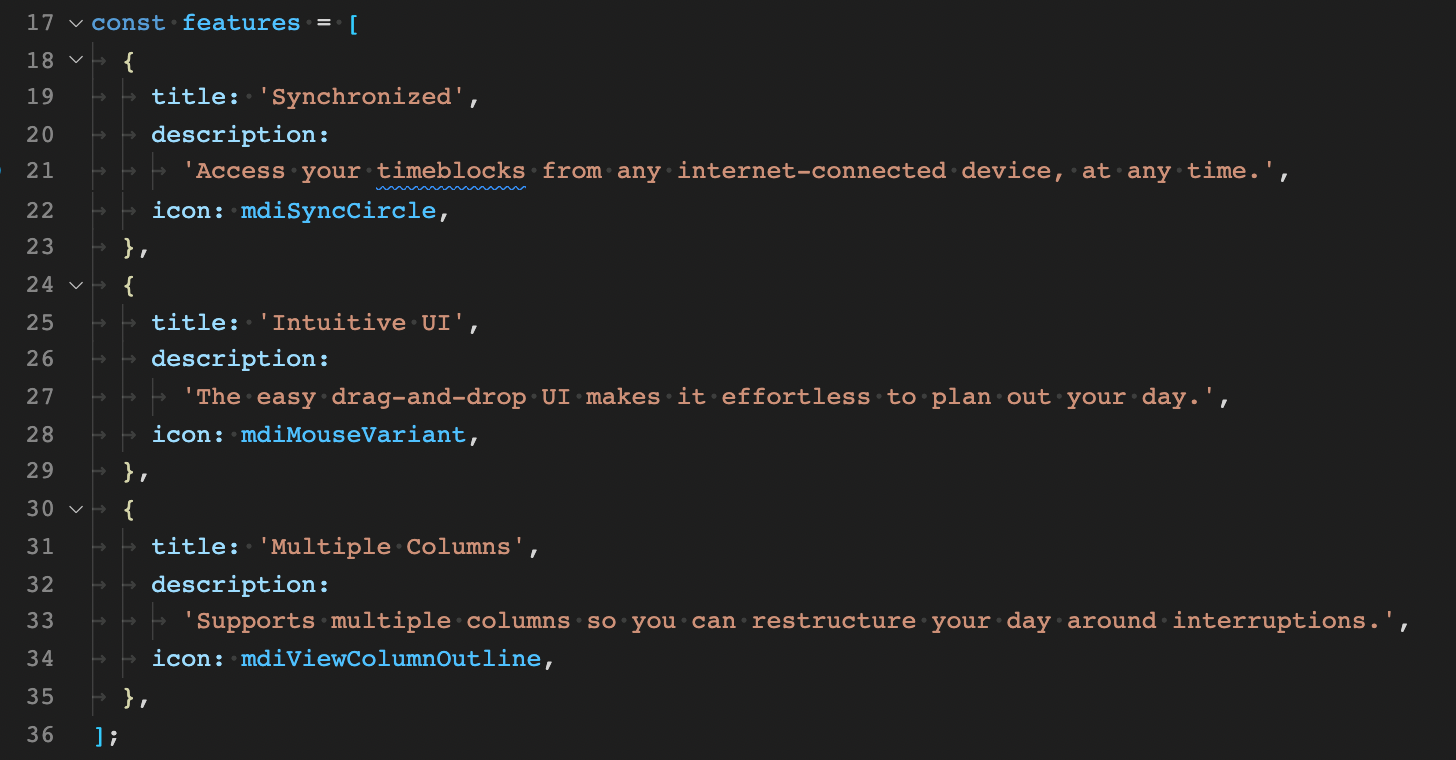
\includegraphics[width=\textwidth]{landing-page-features.png}
\end{figure}

\begin{figure}[H]
	\caption{Rendering the landing page features using Vue's equivalent of a for loop.}
	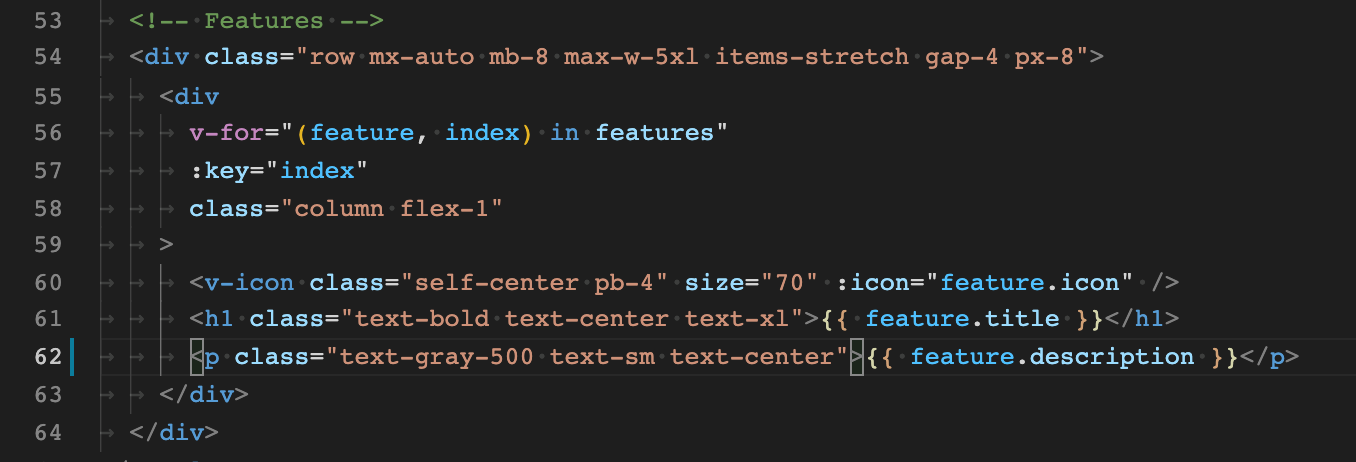
\includegraphics[width=\textwidth]{landing-page-v-for.png}
\end{figure}

\newpage

In addition, I used an if statement for the functionality of the "Create Timeblock" button so that if the use is logged in, it brings them to the "Timeblock" page and otherwise to the "Register" page.
\begin{figure}[H]
	\centering
	\caption{Using an if statement to dynamically redirect the user.}
	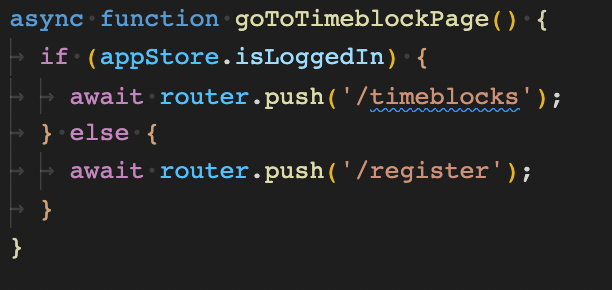
\includegraphics[width=\textwidth]{landing-page-go-to-timeblock-page.png}
\end{figure}

\newpage
\section*{Register/Login Page}

\begin{figure}[H]
	\centering
	\caption{Screenshots of the Register and Login pages, respectively.}
	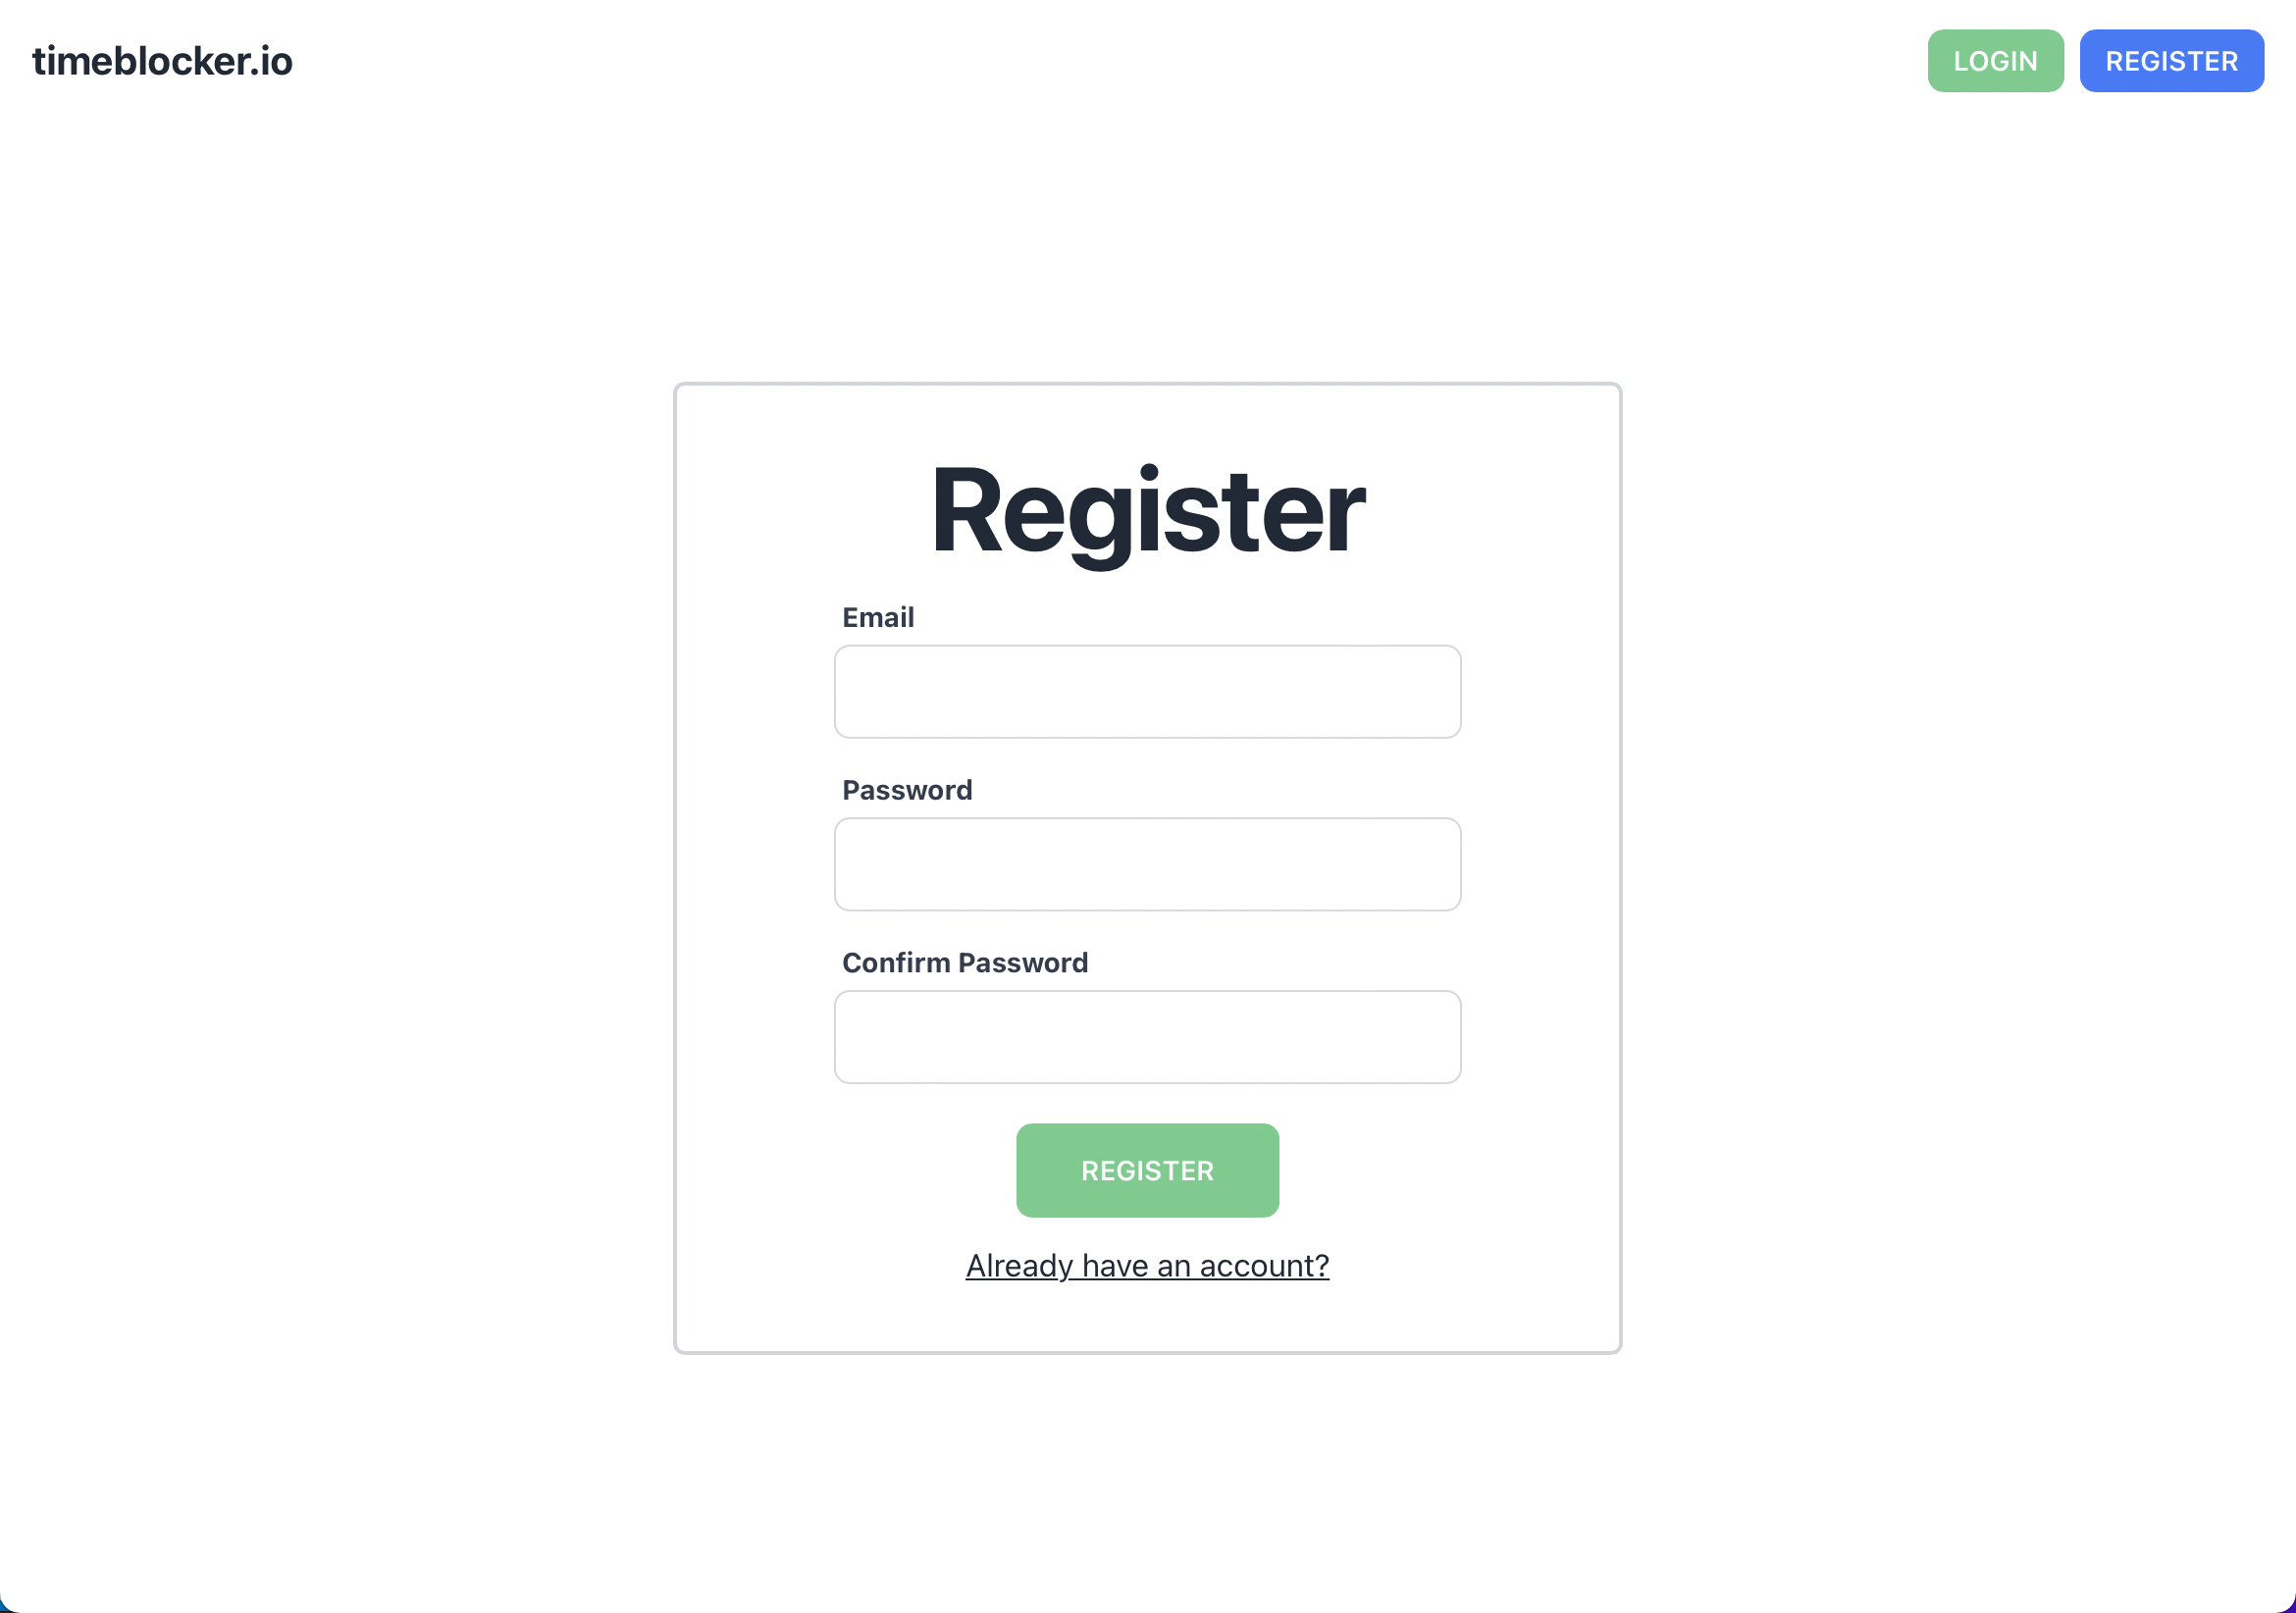
\includegraphics[width=0.7\textwidth]{frontend-register-page.png}
	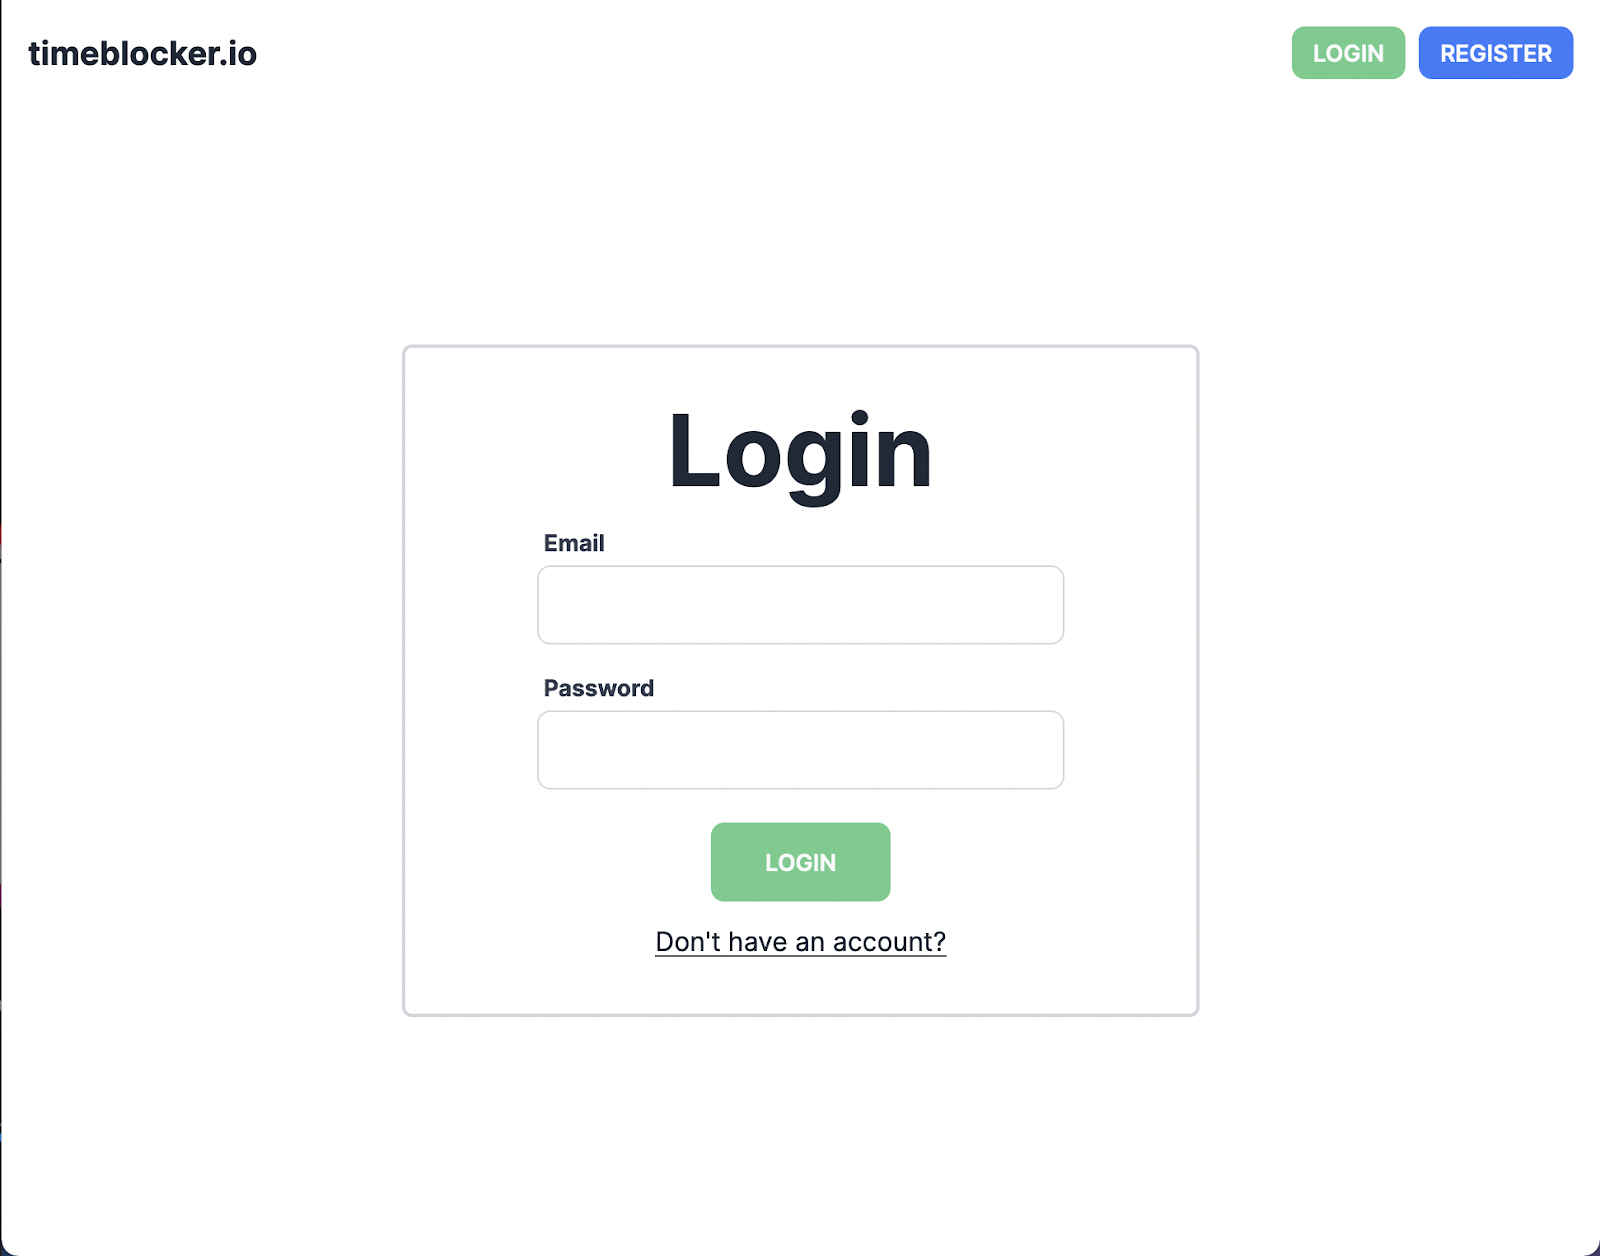
\includegraphics[width=0.7\textwidth]{frontend-login-page.png}
\end{figure}

The register and login pages contain a basic form that prompts them to enter their email and password. Even though they may look like two separate pages, I actually only used one file to create both these pages since they share a lot of code, and I used the current page's route (either \code{/login} or \code{/register}) to decide which form to display:

\begin{figure}[H]
	\centering
	\caption{An example of code reuse: I'm always displaying the password input because both the login and register form require a password, but I'm only displaying the Confirm Password input when the register form is active.}
	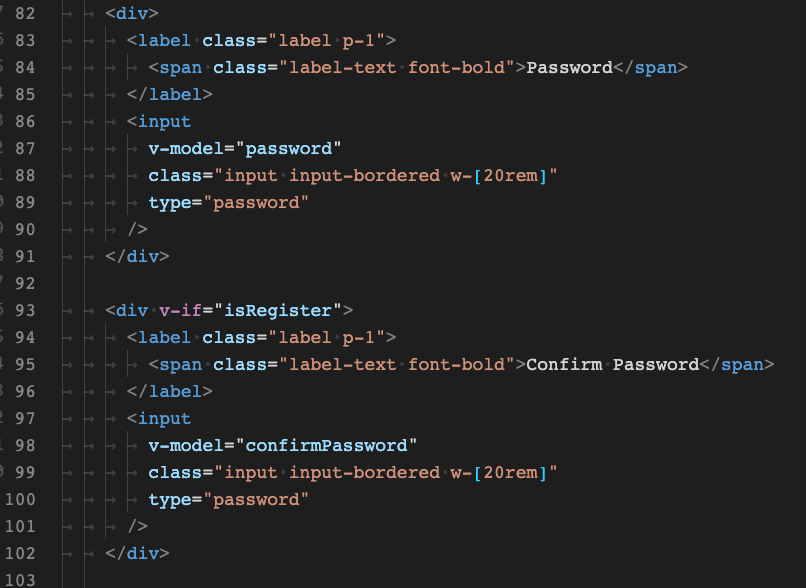
\includegraphics[width=\textwidth]{passwords.png}
\end{figure}

\begin{figure}[H]
	\centering
	\caption{Using Vue's \code{\$computed} function that automatically updates the value of \code{isLogin} whenever the webpage's route changes (which is stored in the \code{route} variable. This way, my page will automatically re-render the correct form whenever the user navigates from the login page to the register page and vice-versa.}
	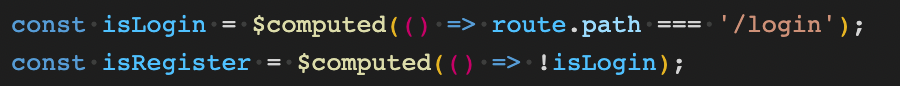
\includegraphics[width=\textwidth]{frontend-entry-page-route.png}
\end{figure}

Once a user clicks the Login button, the \code{login} function is called:

\begin{figure}[H]
	\centering
	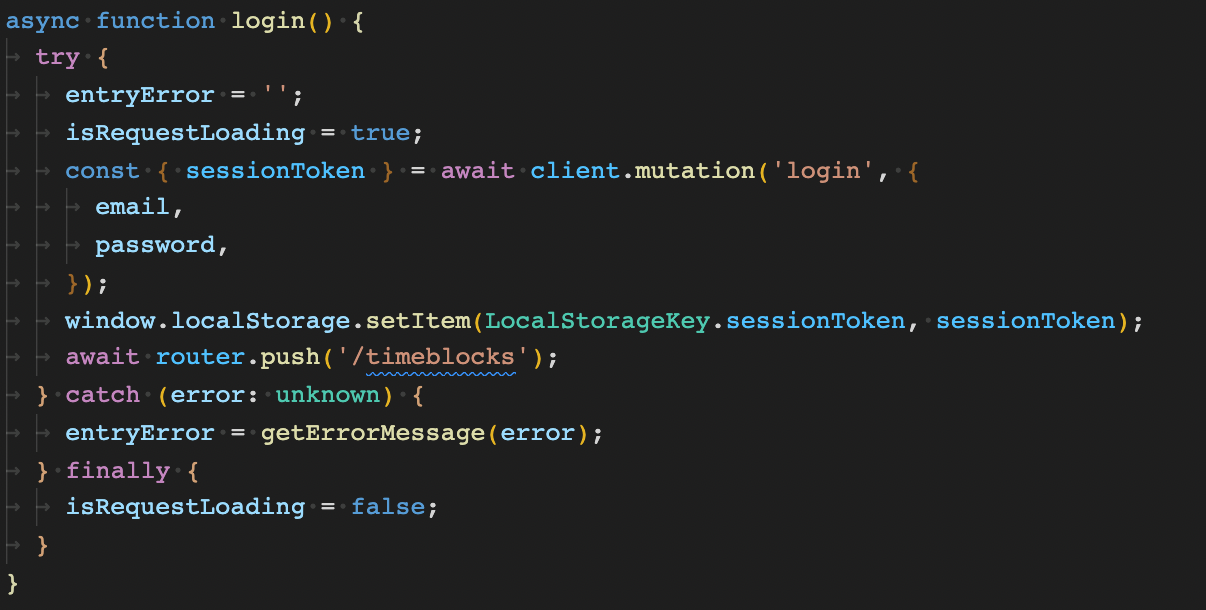
\includegraphics[width=\textwidth]{frontend-login-function.png}
\end{figure}

This function sets the variable \code{isRequestLoading} to true so that the loading spinner displays on the button. It then sends a request to the Node.js backend, which securely deals with user authentication.

\newpage

\section*{Authentication}

When the user creates an account, the frontend makes a request to the backend with the user's email and password and executes the following \code{register} mutation:

\begin{figure}[H]
	\centering
	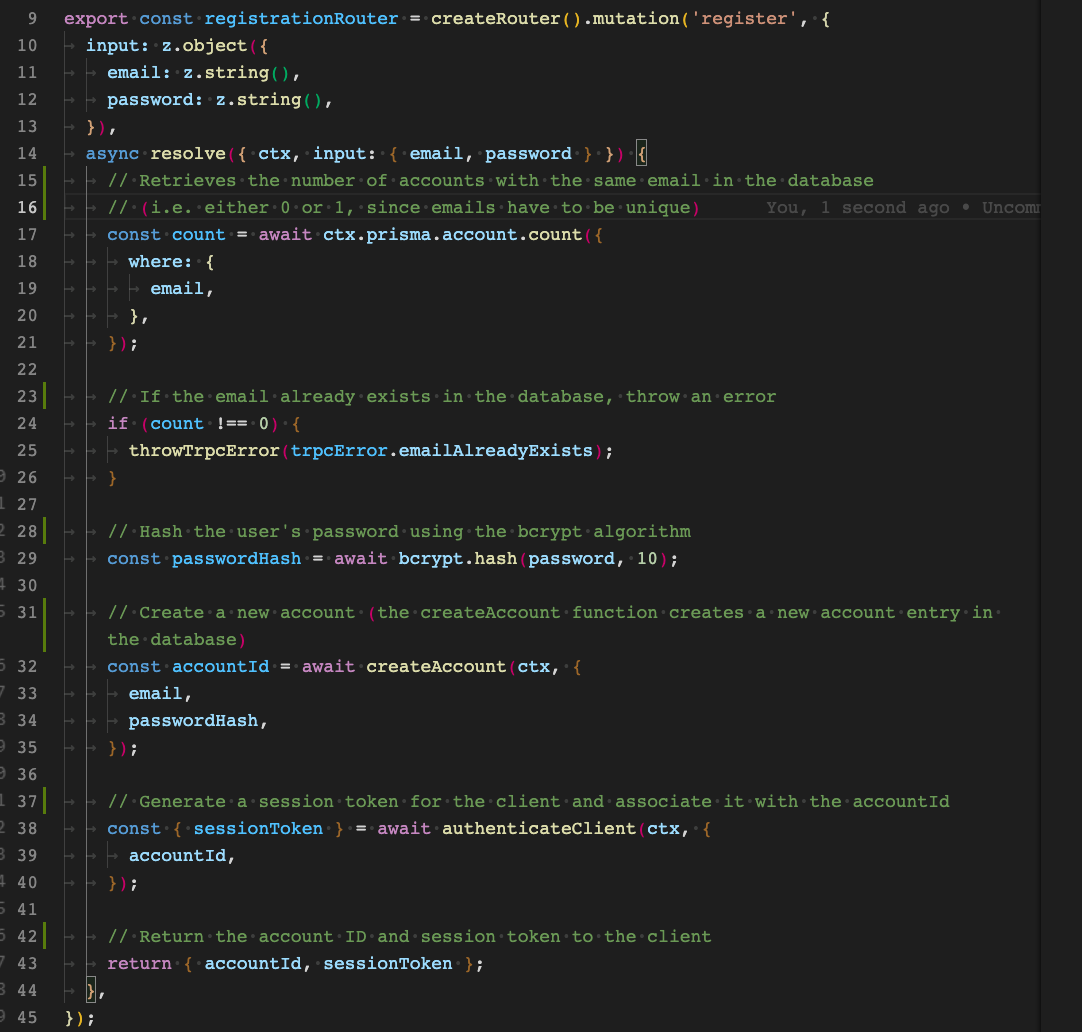
\includegraphics[width=\textwidth]{registration-router.png}
\end{figure}

I decided to store the user's password as a bcrypt hash because retrieving the user's original password from a bcrypt hash is computationally infeasible. This means that if the info from my database were to get leaked, attackers wouldn't be able to easily retrieve the users' original passwords. However, I can still verify whether the user typed in the correct password because two strings that are the same will always produce the same hash, which is how the following login code in the backend words:

\begin{figure}[H]
	\centering
	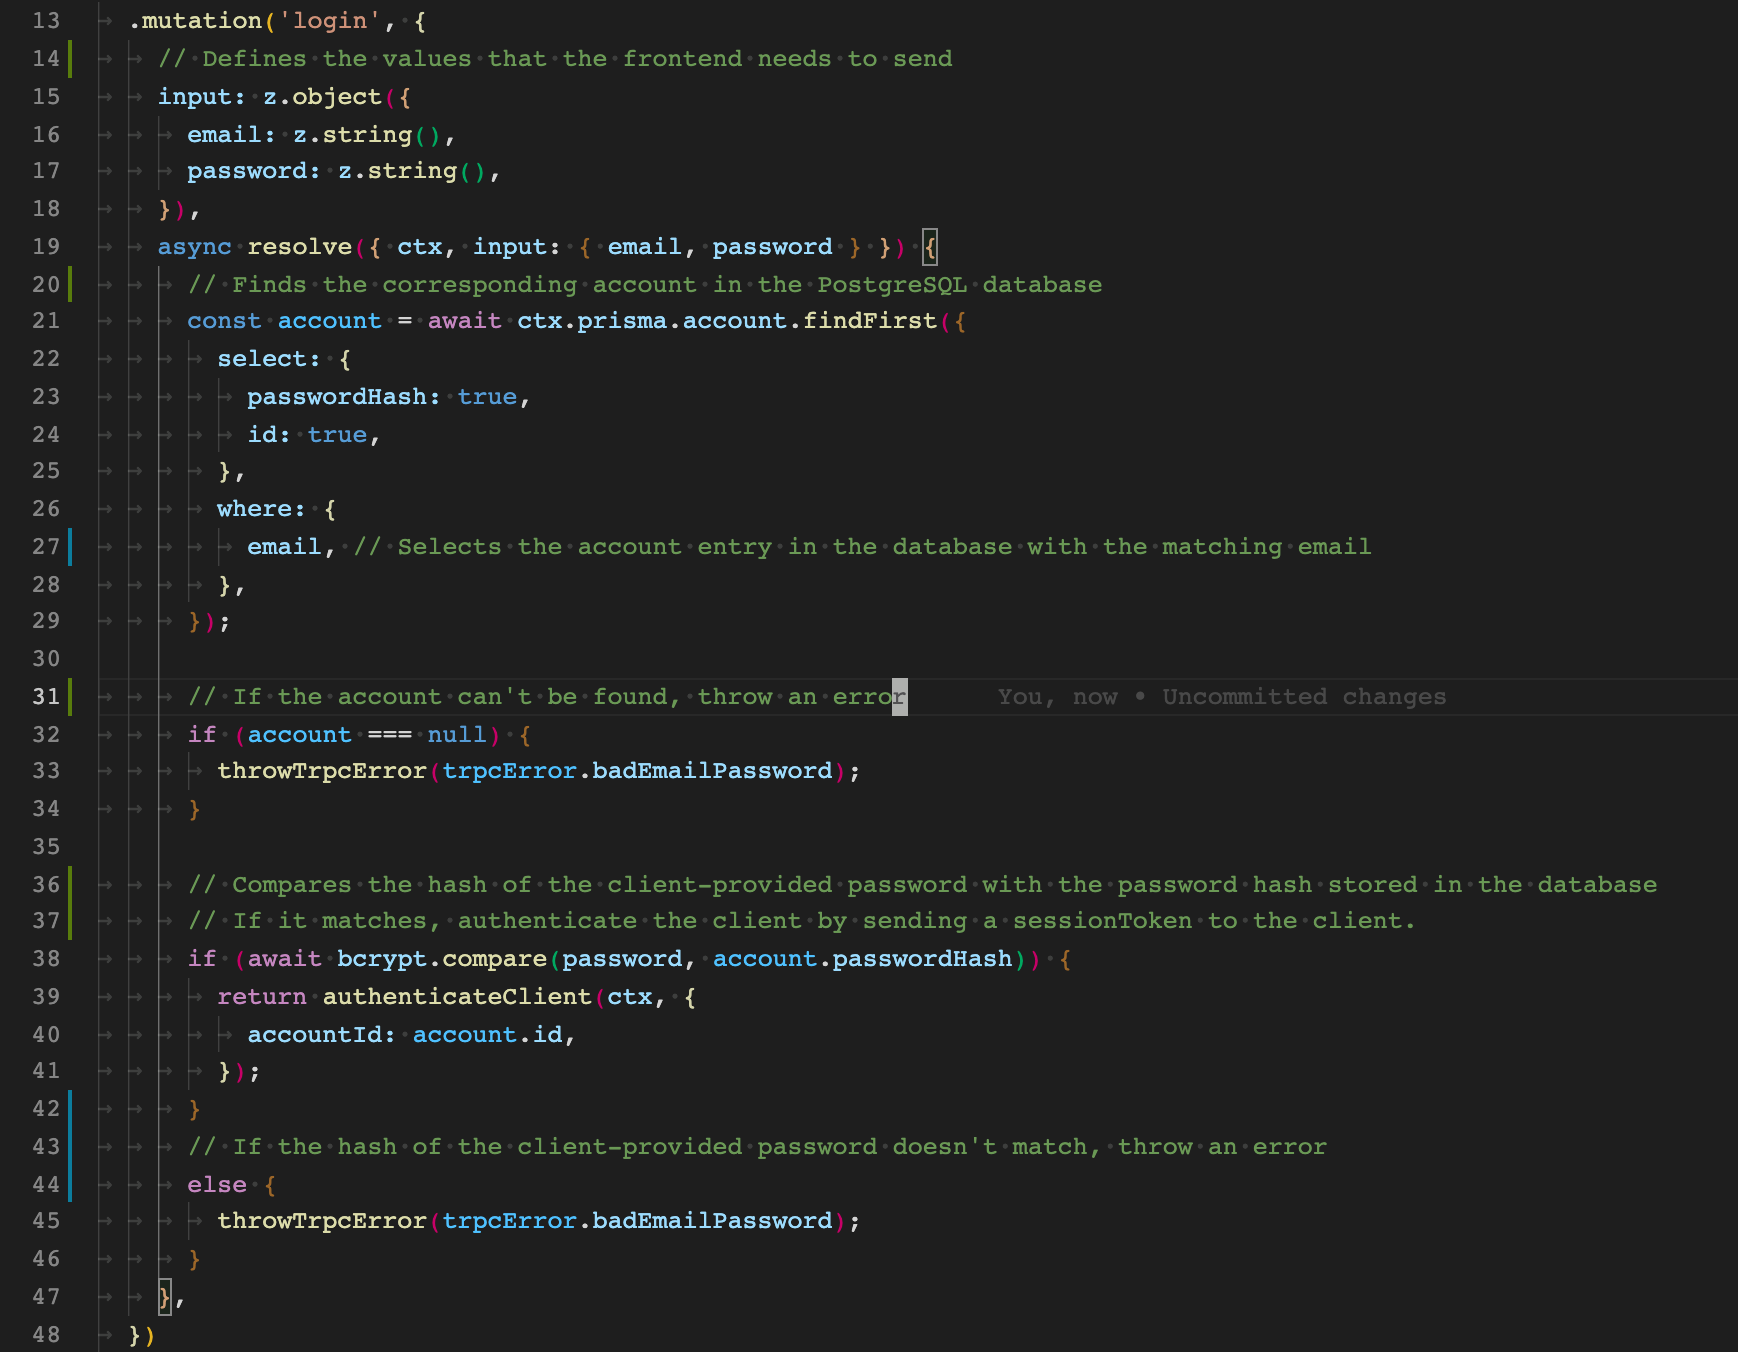
\includegraphics[width=\textwidth]{backend-login-function.png}
\end{figure}

The backend hashes the password entered by the user from the login page, and if the hash matches with the hash in the database, it means that the two passwords are the same and authenticates the client using the following function:

\begin{figure}[H]
	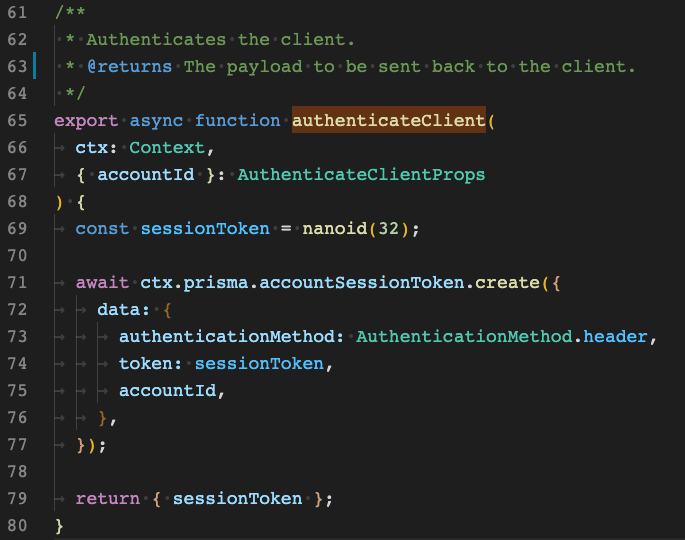
\includegraphics[width=\textwidth]{authenticate-client.png}
\end{figure}

In this function, the backend generates a cryptographically secure and unguessable  session token using \texttt{nanoid} and associates it with the account's ID before saving it to the database. The token is sent back to the client, and the client will send this session token in the HTTP headers with every subsequent request:

\begin{figure}[H]
	\caption{The client is configured to automatically append this token to the \texttt{Authorization} header on every request.}
	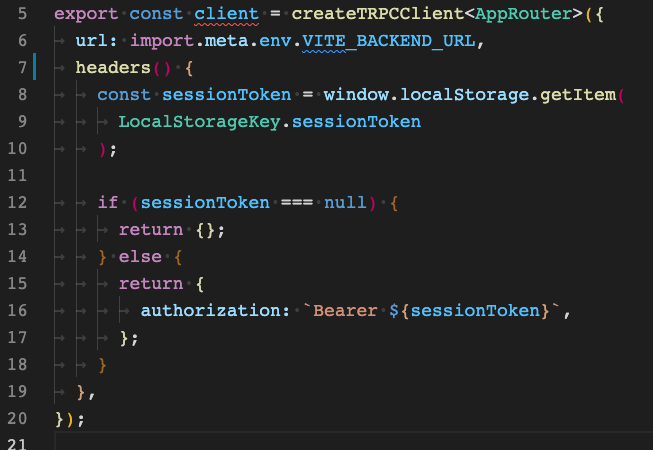
\includegraphics[width=\textwidth]{trpc-headers.png}
\end{figure}

\newpage

Then, the backend will read the value of the \code{Authorization} header with every new request:

\begin{figure}[H]
	\caption{Whenever the user sends a request that needs authentication, this function is called that attempts to read the session token from the header, checks the database for the matching session token and retrieve the account ID associated with the token.}
	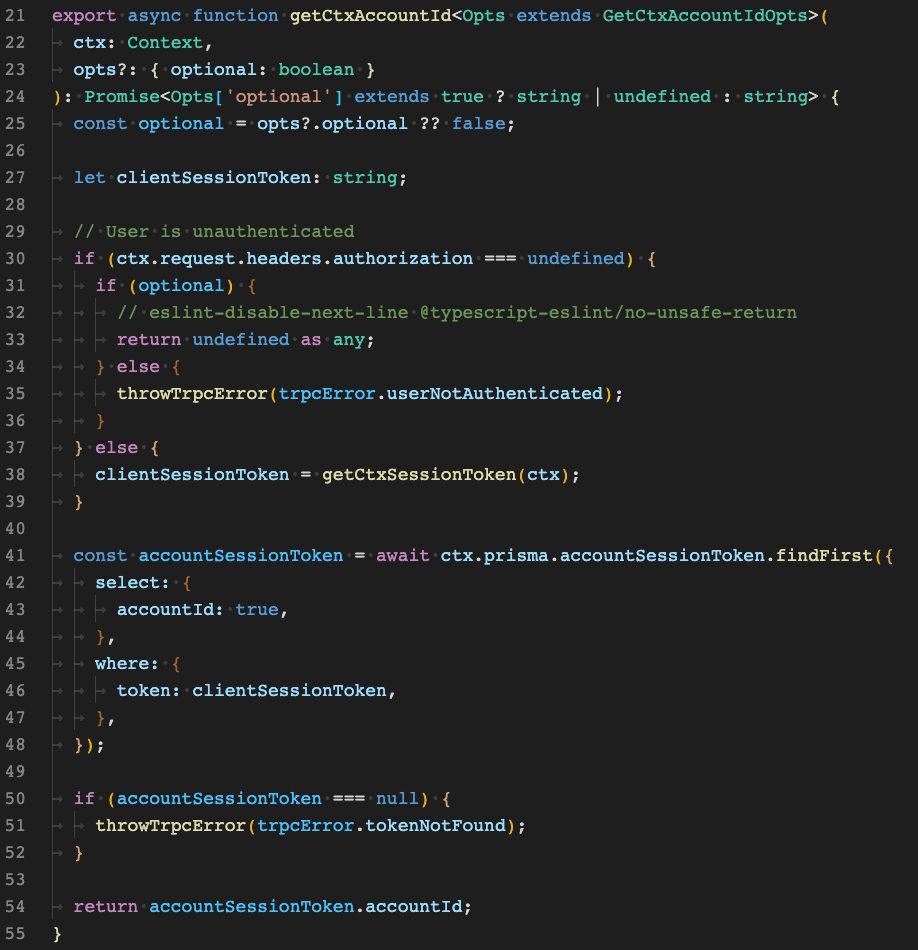
\includegraphics[width=\textwidth]{authentication.png}
\end{figure}

\newpage

\section*{Timeblock Sidebar}

\begin{figure}[H]
	\centering
	\caption{A screenshot of the sidebar with all the user's tasks.}
	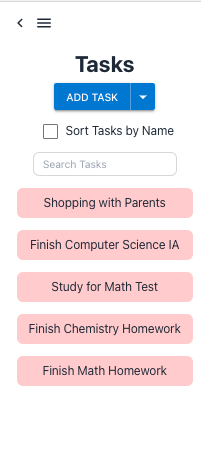
\includegraphics[width=0.5\textwidth]{sidebar.png}
\end{figure}

\newpage

When the user checks the ``Sort Tasks by Name'' checkbox, the tasks are sorted using a recursive merge sort algorithm:

\begin{figure}[H]
	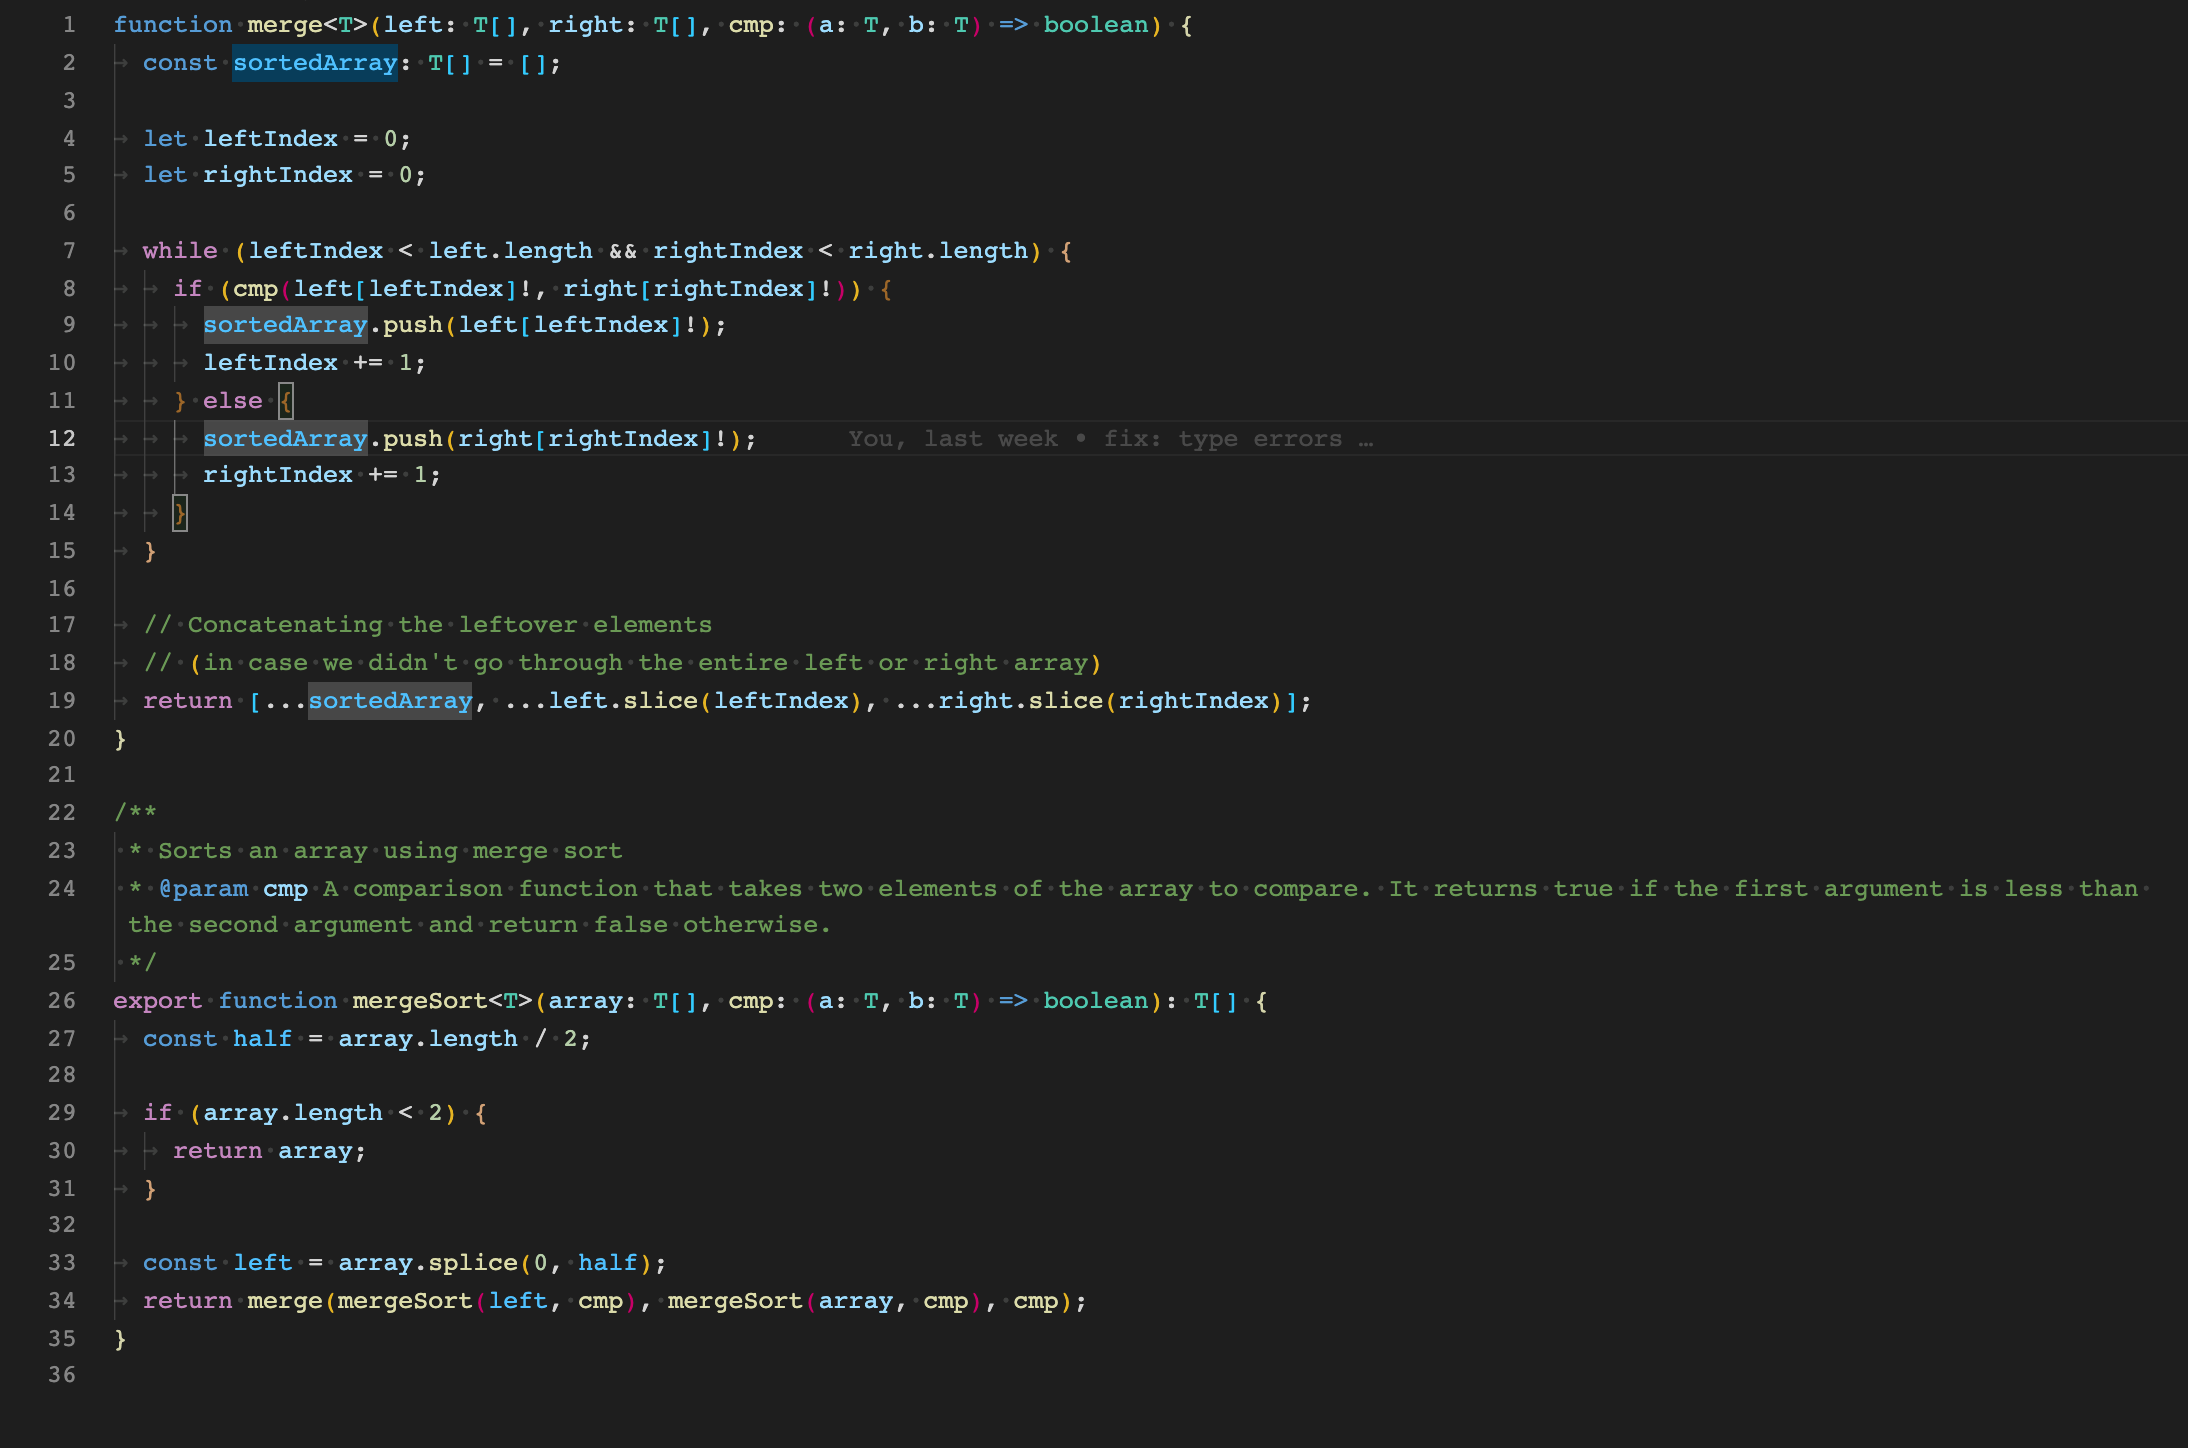
\includegraphics[width=\textwidth]{merge-sort.png}
\end{figure}

\begin{figure}[H]
	\centering
	\caption{The taskbar with tasks sorted by name.}
	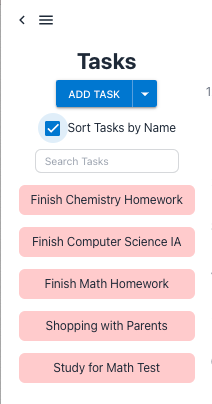
\includegraphics[width=0.3\textwidth]{sorted-taskbar.png}
\end{figure}

Whenever the user types in the ``Search Tasks'' input box, the following code gets executed which uses JavaScript's \code{filter} function to only select the tasks that have a name or description matching the user's input. By converting all strings to lowercase, a case-insensitive search is performed:

\begin{figure}[H]
	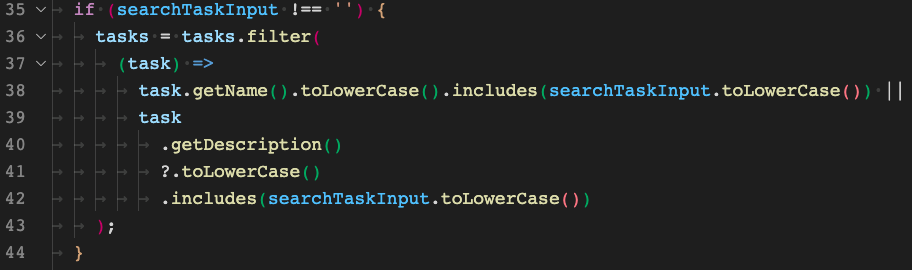
\includegraphics[width=\textwidth]{filtering-tasks.png}
\end{figure}

\newpage

In addition, the sidebar can contain different types of tasks (normal, fixed time, and fixed weekly time tasks). To represent these different tasks, I used inheritance by extending the base Task and TaskBlock classes:

\begin{figure}[H]
	\centering
	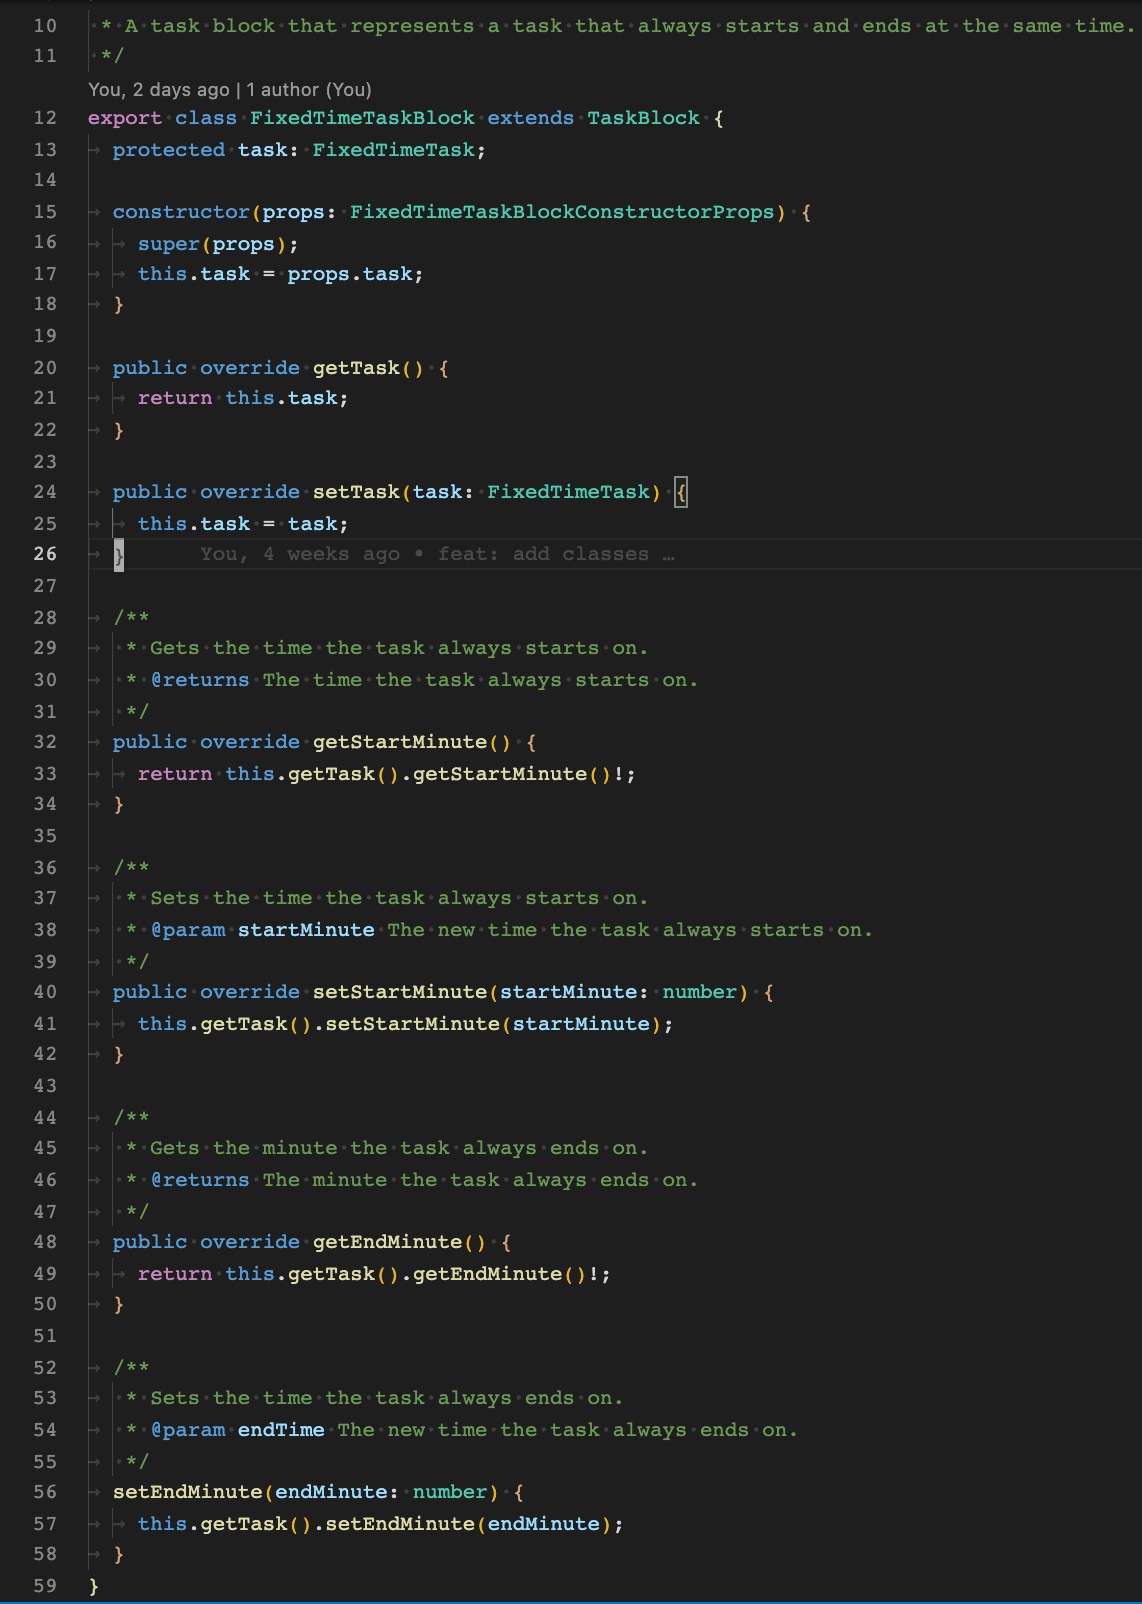
\includegraphics[width=0.9\textwidth]{inheritance.png}
\end{figure}

The FixedTimeTaskBlock class overrides the \code{getStartTime} and \code{getEndTime} methods of the base TaskBlock class. For the FixedTimeTaskBlock class, the start time and the end time are stored in the FixedTimeTask class that the task block is linked to, hence it returns the start time and end time of the task instead. By using inheritance and method overriding, I'm able to leverage polymorphism, as shown in the following code:

\begin{figure}[H]
	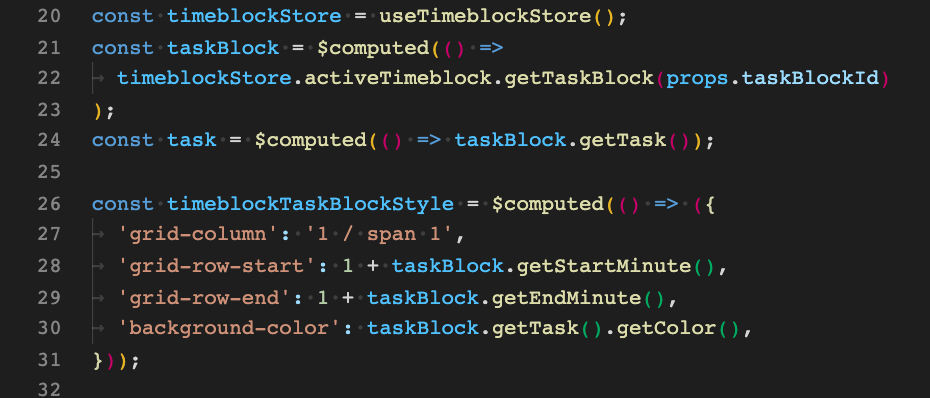
\includegraphics[width=\textwidth]{polymorphism.png}
\end{figure}

\begin{sloppypar}
	In the above code, I'm retrieving the task block using the Timeblock class method \code{getTaskBlock(taskBlockId)}. My code doesn't care which type of TaskBlock it is; the TaskBlock just needs to have a \code{getStartMinute} and \code{getEndMinute} function. When the task block is a FixedTimeTaskBlock, the \code{getStartMinute} and \code{getEndMinute} of the FixedTimeTaskBlock class will be called instead of the \code{getStartMinute} and \code{getEndMinute} of the base TaskBlock class.
\end{sloppypar}

\newpage

\section*{Timeblock Columns}

\begin{figure}[H]
	\caption{Timeblocker supports multiple columns in case your original schedule gets interrupted.}
	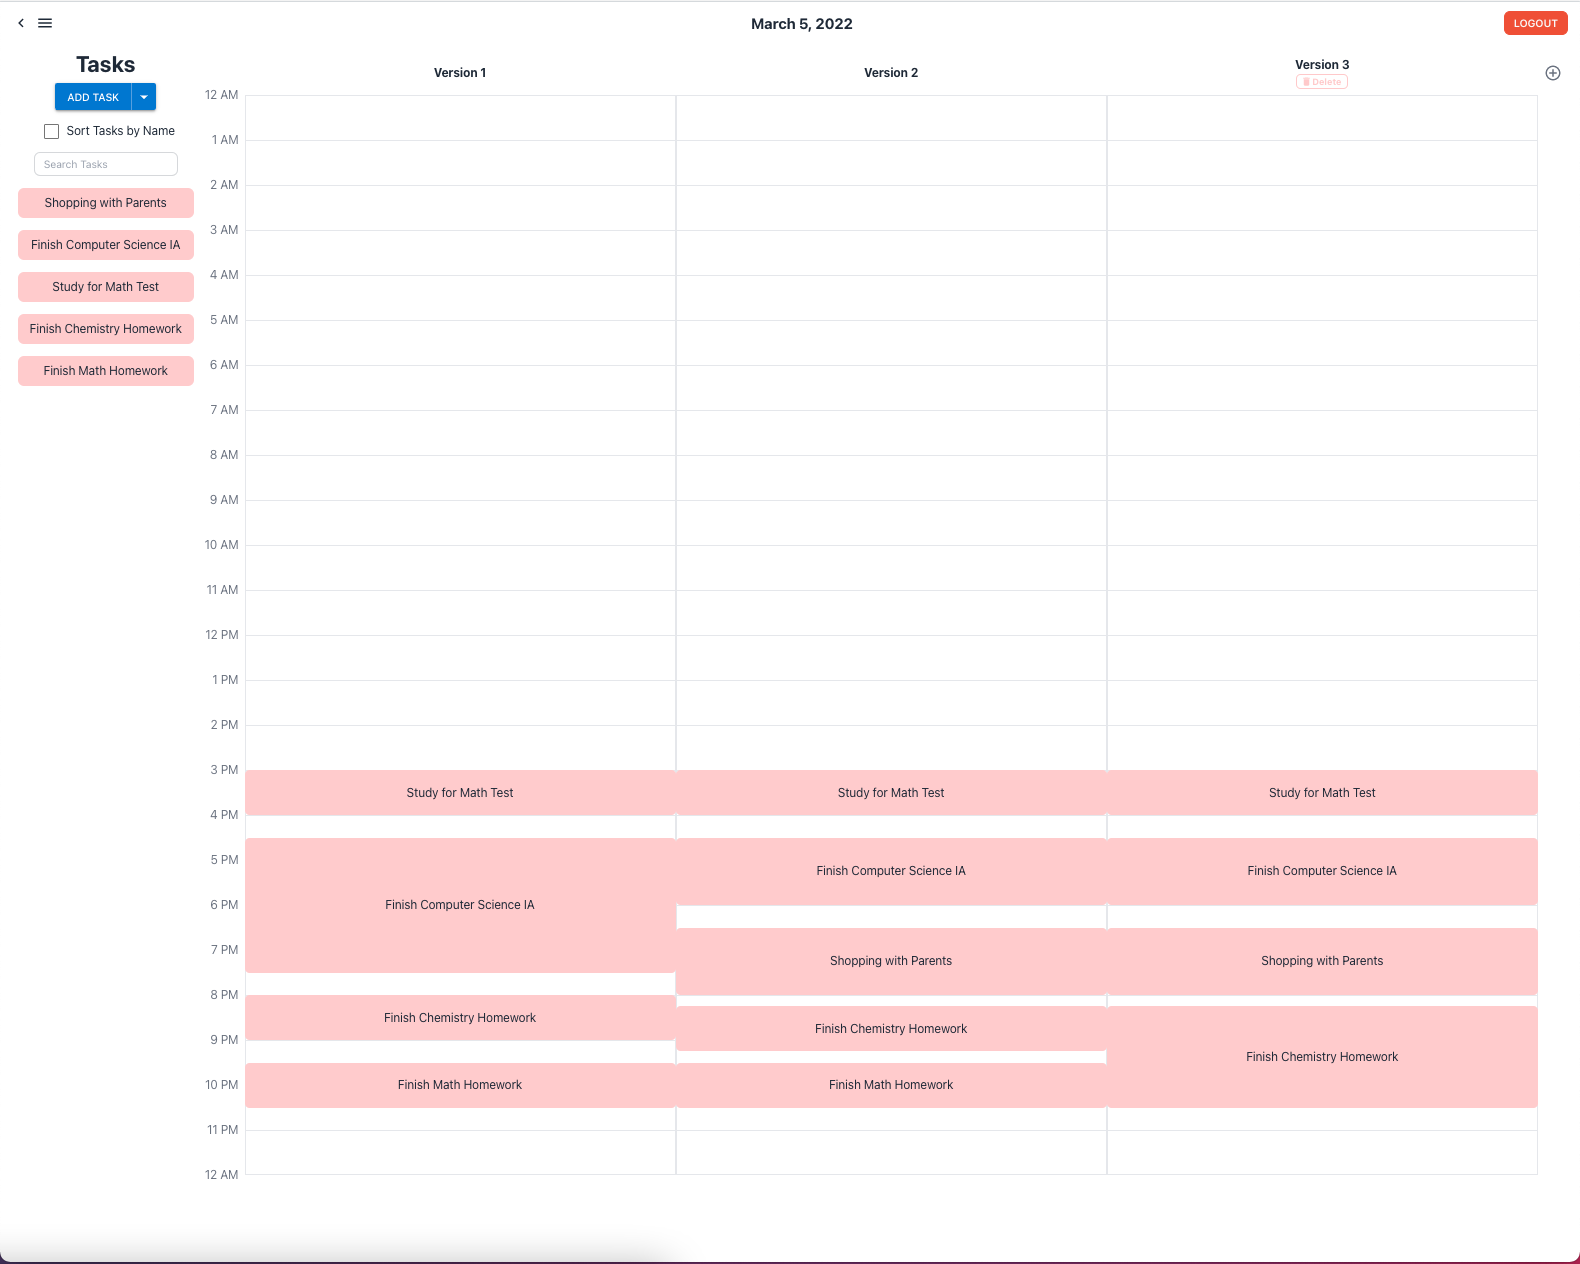
\includegraphics[width=\textwidth]{columns.png}
\end{figure}

When the user creates a new column, all the task blocks on the rightmost column get duplicated and added to the new column. To do this, I used a for-loop that loops through the current columns' task blocks:

\newpage

\section*{Backend}
The backend uses tRPC, a TypeScript library for defining type-safe server routes, and Fastify, a low overhead web framework for Node.js. Significant files/folders include:

\noindent\begin{xltabular}{\textwidth}{
		@{}
		p{0.3\textwidth}
		X
	}
	\adjustbox{valign=t}{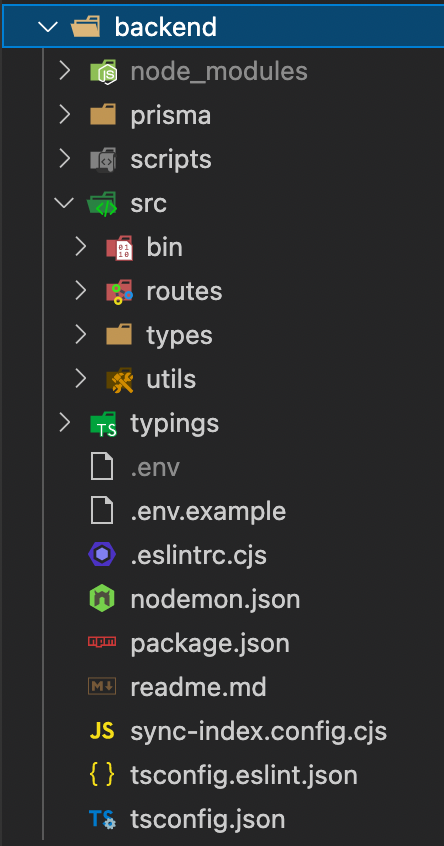
\includegraphics[width=0.3\textwidth]{backend-files.png}}
	&
	\begin{itemize}[label={}, leftmargin=5pt]
		\item	\textbf{prisma/:} Database models and configuration files for the Prisma ORM.
		\item	\textbf{src/:} Main backend source code.
		\item	\textbf{bin/:} Scripts that should be executed to start the server.
		\item	\textbf{routes/:} tRPC route definitions.
		\item	\textbf{types/:} TypeScript types.
		\item	\textbf{utils/:} Various utility functions.
		\item	\textbf{.env:} Environment secrets (should not be public!)
		\item	\textbf{Configuration files (*.cjs, *.json):} Configuration files for various backend development tools.
	\end{itemize}
\end{xltabular}

\newpage

\section*{Starting the Server}

\begin{figure}[H]
	\caption{The code that is executed to start the server. \code{dayjs} is a date manipulation library for JavaScript that supports timezones, which is crucial for ensuring that fixed weekly time tasks repeat on the same weekdays.}
	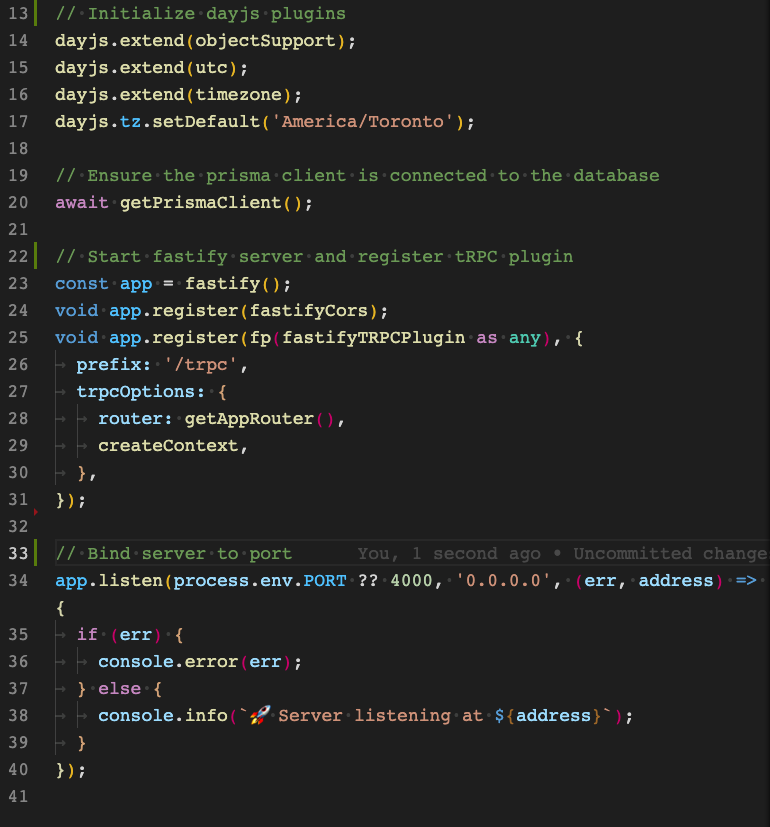
\includegraphics[width=\textwidth]{server-start.png}
\end{figure}

\newpage

\section*{Database}

To synchronize the user's data across different devices, the user's data is stored in a PostgreSQL database in the cloud. The server interacts with this database using the Prisma ORM, which provides type-safe functions to query the database and protects against SQL vulnerabilities by default:

\subsection*{Database Models}

\begin{figure}[H]
	\caption{The database models I created for the Prisma ORM. Prisma takes these models and generates the corresponding TypeScript types that give me type safety when interacting with the database.}
	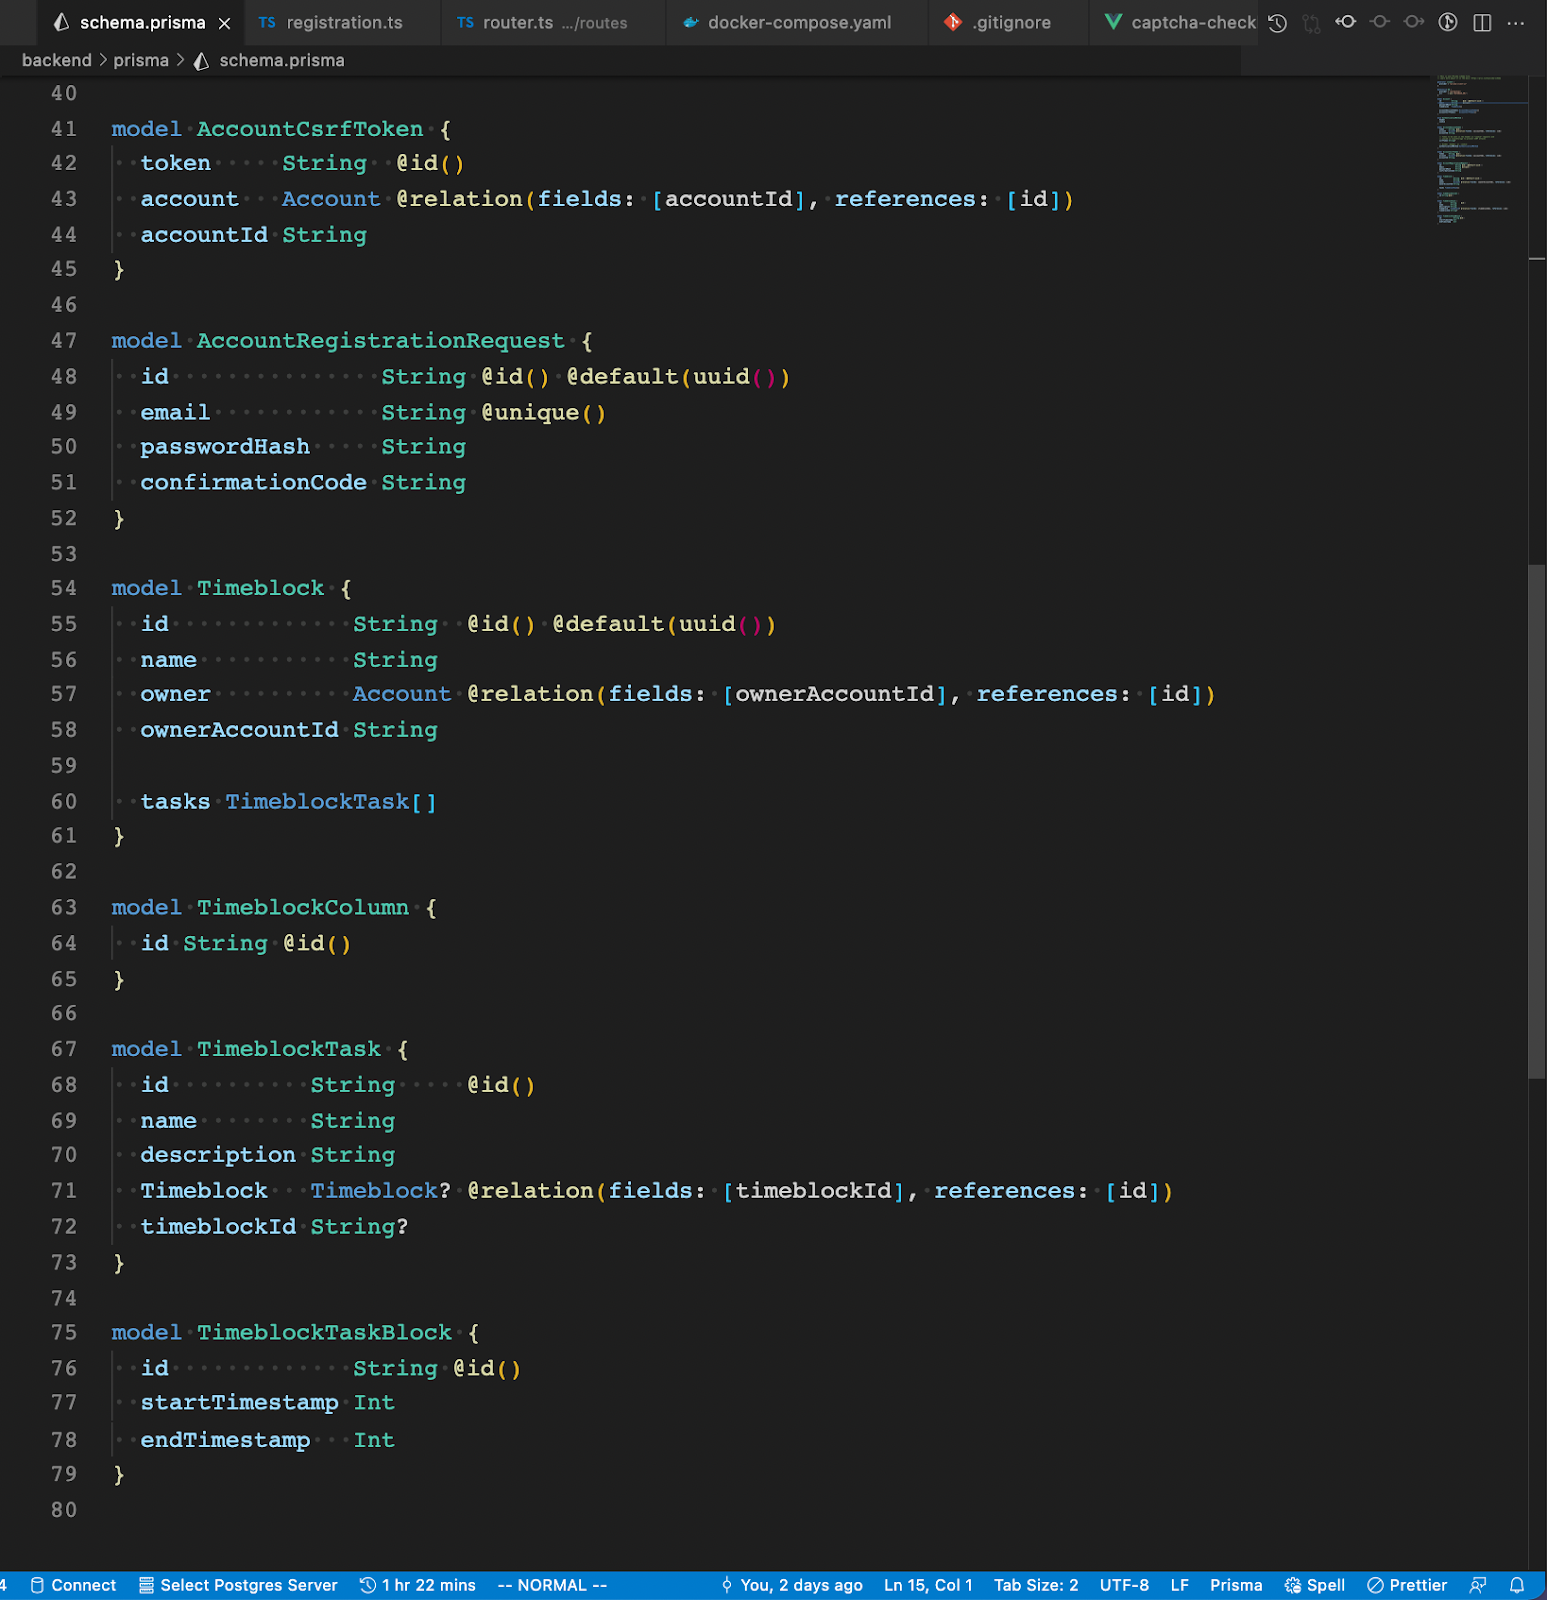
\includegraphics[width=1\textwidth]{backend-database-models.png}
\end{figure}

\newpage

\section*{tRPC Routes}

The backend routes are defined using the tRPC library:

\begin{figure}[H]
	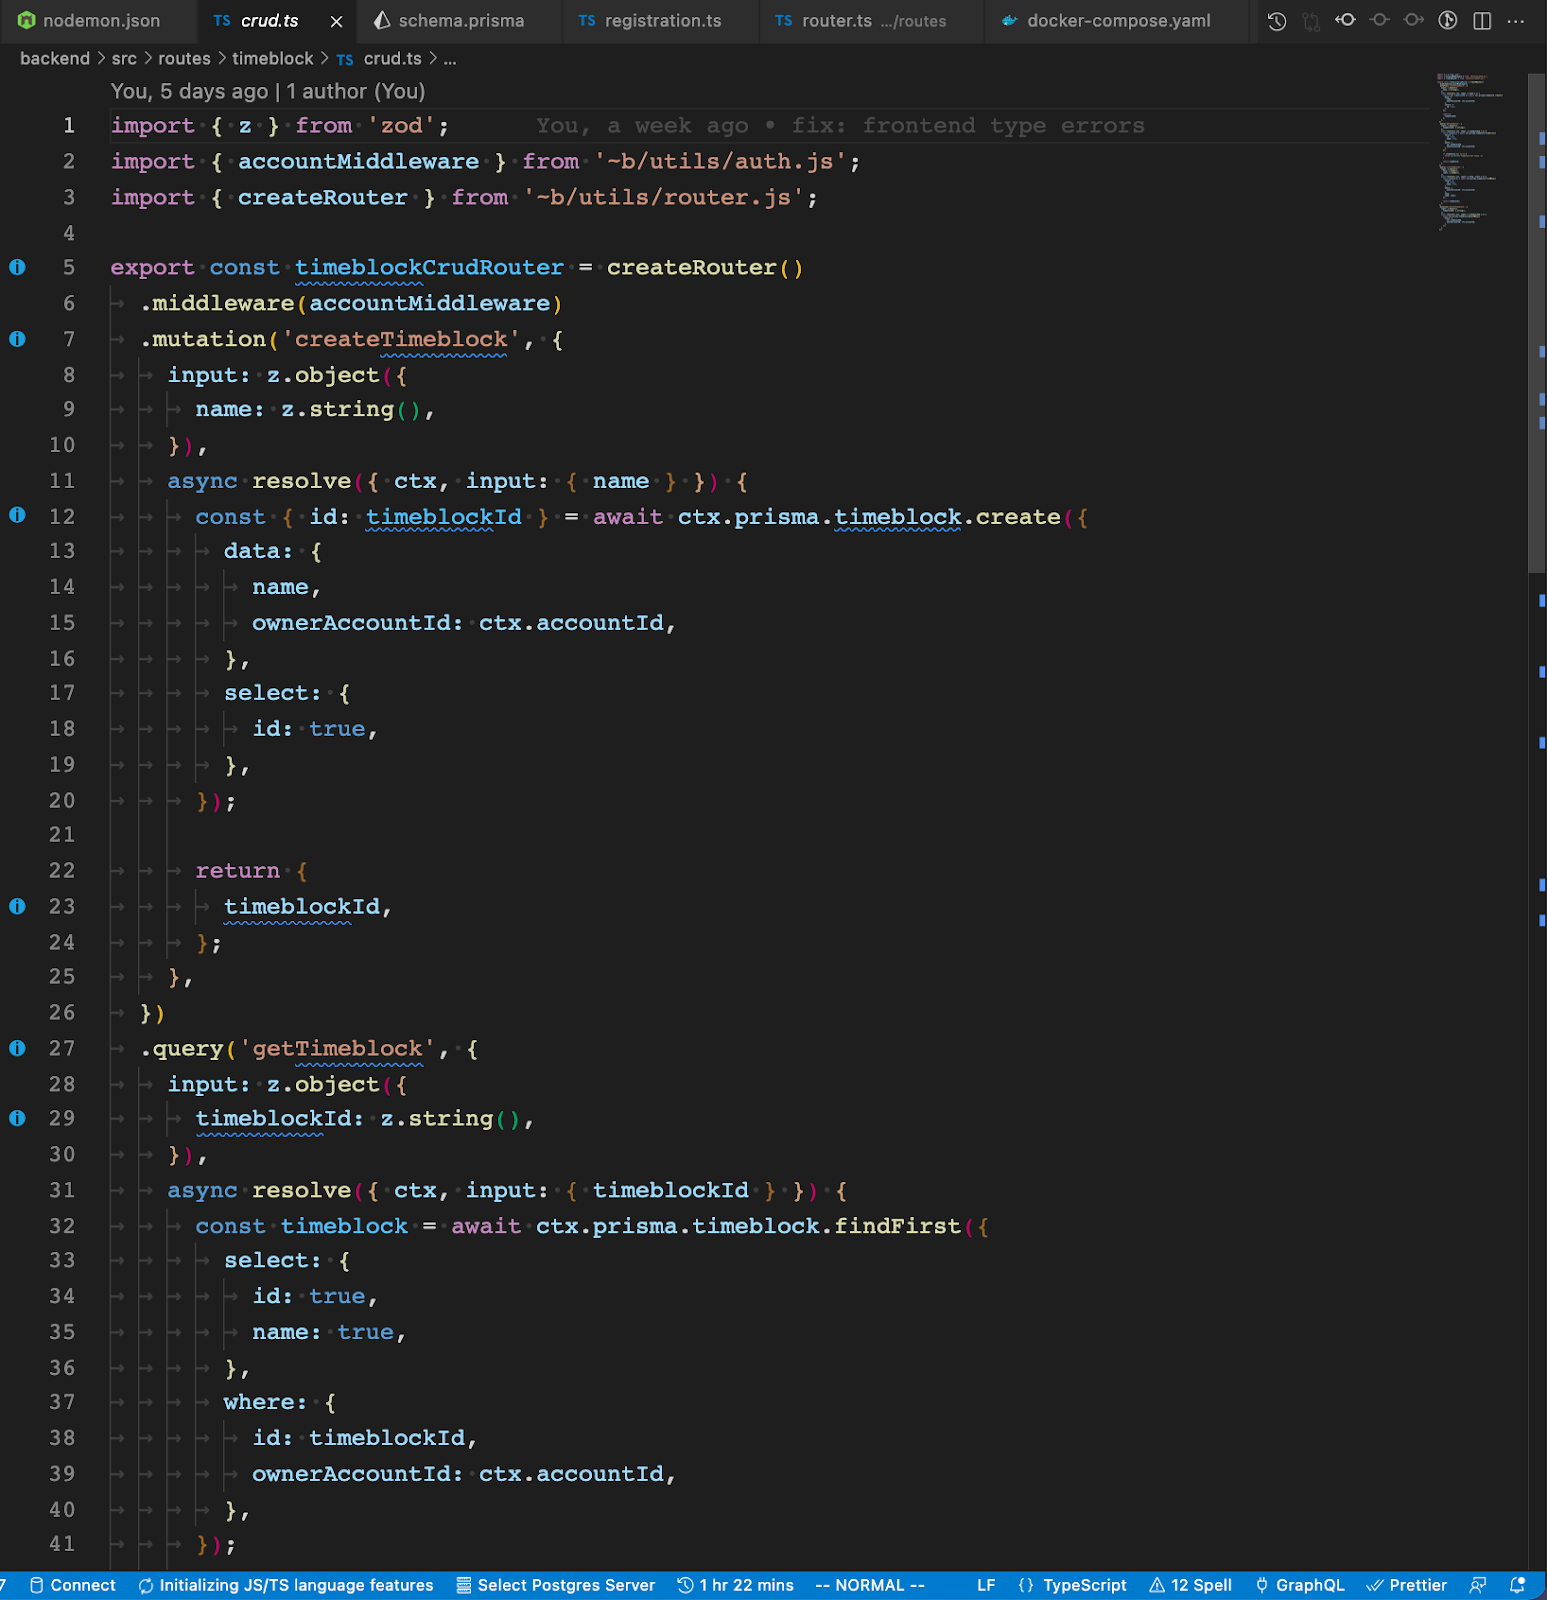
\includegraphics[width=1\textwidth]{backend-trpc-routes.png}
\end{figure}

\begin{sloppypar}
	The tRPC library supports custom middleware; in the above code, I'm using my own \code{accountMiddleware} that ensures the user is authenticated by checking if they have the \code{Authorization} header set to a valid session token. Then, I'm creating the \code{getTimeblock} query that takes an object with the timeblock ID and then defining the \code{resolve} function that locates the timeblock in the PostgreSQL database using Prisma's \code{findFirst} function and returning it to the client if found.
\end{sloppypar}

\newpage

\def\arraystretch{1.3}
\section*{Solution Mastery Aspect}
\textbf{IB Standard Level}
\vspace{-6pt}
\noindent\begin{xltabular}{\textwidth}{|p{0.3\textwidth\RaggedRight}|X|}
	\hline
	\textbf{Mastery Factor}
	& \textbf{Where it would be used}
	\\\hline
	1. Arrays
	& Array of tasks in the schedule
	\\\hline
	2. User-defined objects
	& A list of task blocks
	\\\hline
	3. Objects as data records
	& Task box details (title, description, etc.).
	\\\hline
	4. Simple selection (if-else)
	& When the user creates a task, an if statement is used to check if the task name is empty, and if so, cancels creating the task (since a task's name can't be empty).
	\\\hline
	5. Complex selection (nested if, if with multiple conditions or switch)
	& When the user has selected the type of task to create, I use a switch statement when initializing the correct class instance for the type of task the user is creating.
	\\\hline
	6. Loops
	& Looping through all the task blocks that need to be created on the client-side when the list of the user's task blocks are returned from the server.
	\\\hline
	7. User-defined methods
	& The onDrop method that gets called whenever a user drops a task onto the schedule.
	\\\hline
	8. User-defined methods with appropriate return values
	& A method that returns the color based on the type of task so that the different types of tasks are colour-coded.
	\\\hline
	9. Sorting
	& Sorting of task boxes in the preview based on the task names.
	\\\hline
	10. Searching
	& Searching through task boxes based on the name/description.
	\\\hline
	11. Use of additional libraries
	& I will be using various industry-standard frontend and backend development tools and libraries for making development easier. The main ones are Vue.js (a JavaScript framework for building user interfaces) for the frontend, and Fastify (a fast Node.js web framework) for the backend. See Appendix for a complete list of third-party libraries used in Timeblocker.
	\\\hline
\end{xltabular}

\bigskip

\noindent\textbf{IB Higher Level}
\smallskip

\def\arraystretch{1.5}
\noindent\begin{xltabular}{\textwidth}{|l|X|}
	\hline
	\textbf{Mastery Factor}
	& \textbf{Where it would be used}
	\\\hline
	1. Polymorphism
	& The different types of task blocks and task boxes will have the same method signatures but have different functionality, and I use polymorphism to invoke the unique functionality of each task block.
	\\\hline
	2. Inheritance
	& Specific types of tasks and task blocks (fixed weekly task and fixed weekly time tasks) inherit from the Task and TaskBlock base classes.
	\\\hline
	3. Encapsulation
	& The classes will only expose getters and setters that retrieve private properties on classes. The setters will validate the input to make sure that the new value set on the class instance is valid.
	\\\hline
	4. Database
	& Timeblocker will be using PostgreSQL as the database, using Prisma as the ORM for type-safety with TypeScript.
	\\\hline
\end{xltabular}

\end{document}
